\documentclass[oneside, 12pt]{scrreprt}
\usepackage[german, english]{babel}
\usepackage{lmodern}
\usepackage{amssymb}
\usepackage{amsmath}
\usepackage{amsthm}
\usepackage{dsfont}
\usepackage{bigints}
\usepackage{graphicx}
\usepackage{subcaption}
\usepackage{leftidx}
\usepackage[utf8]{inputenc}
\inputencoding{latin1}
\usepackage[inline]{enumitem}
\usepackage[hyperref,backend=biber,backref,backrefstyle=none]{biblatex}
\usepackage{bbm}
\usepackage[toc]{appendix}
%\usepackage{mcode}
%\usepackage{draftwatermark}
\usepackage{hyperref}
\usepackage{cleveref}
\hypersetup{
    colorlinks=true,
    linkcolor=blue,
    %filecolor=magenta,      
    %urlcolor=cyan,
}

\newtheorem{theorem}{Theorem}[chapter]
\newtheorem{lemma}[theorem]{Lemma}
\newtheorem{remark}[theorem]{Remark}
\newtheorem{example}[theorem]{Example}
\newtheorem{proposition}[theorem]{Proposition}
\newtheorem{definition}[theorem]{Definition}
\newtheorem{corollary}[theorem]{Corollary}
\newtheorem{interpretation}[theorem]{Interpretation}
\newtheorem{assumption}{Assumption}
\newtheorem{notation}{Notation}
\def\figurename{\footnotesize Bild}
\crefname{subsection}{subsection}{subsections}

%\newcommand{\ind}{\vspace*{0.1ex}\underline{\mbox{ } || \mbox{ }}\vspace*{-0.1ex}}
\newcommand{\ind}{\perp\hspace*{-1ex}\perp}
\newcommand{\bN}{\mathbb{N}}
\newcommand{\bZ}{\mathbb{Z}}
\newcommand{\bR}{\mathbb{R}}
\newcommand{\bE}{\mathbb{E}}
\newcommand{\bC}{\mathbb{C}}
\newcommand{\bF}{\mathbb{F}}
\newcommand{\cB}{\mathcal{B}}
\newcommand{\cS}{\mathcal{S}}
\newcommand{\cD}{\mathcal{D}}
\newcommand{\cX}{\mathcal{X}}
\newcommand{\cF}{\mathcal{F}}
\newcommand{\cG}{\mathcal{G}}
\newcommand{\cP}{\mathcal{P}}
\newcommand{\cA}{\mathcal{A}}
\newcommand{\cE}{\mathcal{E}}
\newcommand{\cO}{\mathcal{O}}
\newcommand{\cZ}{\mathcal{Z}}
\newcommand{\cL}{\mathcal{L}}
\newcommand{\cT}{\mathcal{T}}
\newcommand{\cQ}{\mathcal{Q}}
\newcommand{\cIS}{\mathcal{IS}}
\newcommand{\cI}{\mathcal{I}}
\newcommand{\F}{\mathcal{F}}
\newcommand{\halmos}{\quad\hfill\mbox{$\Box$}}
\newcommand{\cov}{\mbox{\rm Cov}\,}
\newcommand{\cor}{\mbox{\rm Cor}\,}
\newcommand{\var}{\mbox{\rm Var}\,}
\newcommand{\supp}{\mbox{\rm supp}\,}
\newcommand{\barR}{\overline{\bR}}
\newcommand{\barB}{\overline{\cB}_1}
\newcommand{\mbb}{\mathbb}
\newcommand{\One}{\mathds{1}}
\newcommand{\RR}{\mathbb{R}}
\newcommand{\BB}{\mathbb{B}}
\newcommand{\VAR}{\mbox{V@R}}
\newcommand{\AVAR}{\mbox{AV@R}}
\newcommand{\one}{\mathds{1}}

\DeclareCiteCommand{\morecite}[\mkbibbrackets]
  {\usebibmacro{prenote}}%
  {\usebibmacro{citeindex}%
   \printnames{labelname}%
   \setunit{\addcomma\space}
   \usebibmacro{cite}}
  {\multicitedelim}%
  {\usebibmacro{postnote}}


\usepackage{listings}
\usepackage{color} %red, green, blue, yellow, cyan, magenta, black, white
\definecolor{mygreen}{RGB}{28,100,0} % color values Red, Green, Blue
\definecolor{mylilas}{RGB}{170,55,241}


\addbibresource{Reference.bib}
\DeclareNameAlias{default}{last-first}
\setcounter{chapter}{0}
%\setcounter{secnumdepth}{0}
\begin{document}

\lstset{language=Matlab,%
    %basicstyle=\color{red},
    breaklines=true,%
    morekeywords={matlab2tikz},
    keywordstyle=\color{blue},%
    morekeywords=[2]{1}, keywordstyle=[2]{\color{black}},
    identifierstyle=\color{black},%
    stringstyle=\color{mylilas},
    commentstyle=\color{mygreen},%
    showstringspaces=false,%without this there will be a symbol in the places where there is a space
    numbers=left,%
    numberstyle={\tiny \color{black}},% size of the numbers
    numbersep=9pt, % this defines how far the numbers are from the text
    emph=[1]{for,end,break},emphstyle=[1]\color{red}, %some words to emphasise
    %emph=[2]{word1,word2}, emphstyle=[2]{style},    
}



\begin{titlepage}

\includegraphics[height=1.8cm]{images/unilogo_bild}
\hfill

\includegraphics[height=1.8cm]{images/unilogo_wort}\\[1em]

\pagenumbering{gobble}
\thispagestyle{empty}
\textwidth28cm
\begin{center}
{\Large\bfseries Ulm University\\
   Faculty of Mathematics and Economics\\
}
\vspace{3cm}
{\LARGE\bfseries
An Euler-Poisson Scheme for L\'evy driven Stochastic Differential Equations
\\
}
\vspace{1cm}
{\Large
Master's Thesis} \\
\bigskip % nach löschen dieser Zeile ein \bigskip einfügen.
{\Large in Finance}
\end{center}
\vspace{1.5cm}
\begin{center}
by \\
$\mbox{Odunayo O. Rotimi}$ \\
$\mbox{August 19, 2019}$\\

\vspace*{1.2cm}
\textbf{ Advisors} \\

$\mbox{Prof. Dr. Robert Stelzer}$\\
$\mbox{Prof. Dr. Mitja Stadje}$
\end{center}
\vfill
\end{titlepage}
${ }$
\let\cleardoublepage\clearpage
%\newpage

%\chapter*{Dedication}
%To Jesus Christ, the source of all refreshing in a dry and thirsty land.
 

\thispagestyle{empty}
\setcounter{page}{0}
\tableofcontents
\clearpage

\pagenumbering{arabic}
\setcounter{page}{1} \normalsize
\chapter{Introduction}
\section{Preview}
Stochastic differential equations play important roles in modeling quantitative phenomena. Their field of application includes but is not limited to: Physics \morecite{feller1951diffusion}, Biometrics \morecite{barndorff2012levy}, modeling contingencies in Actuarial Sciences as well as valuation of financial instruments and entities in the field of Finance \morecite{black1973pricing}. Particularly, the ever evolving nature of financial markets around the world is synchronized with an increase in its risk characteristics, which requires the use of sophisticated models that are robust enough to capture such dynamics; hence the prominence of  L\'evy driven stochastic differential equations in the discipline of Financial Mathematics; see for example, \morecite{tankov2003financial}.

In this thesis, we are interested in the discrete approximation of the stochastic process \break $Y=(Y_t)_{t \in [0, T]}$; defined on the filtered probability space $(\Omega , \mathcal{F}, (\mathcal{F}_t)_{t \geq 0}, \mathcal{P})$; which is the strong solution to
\begin{equation}\label{first_eq}
      Y_t = y_0  + \int_0^t a(Y_{s-})dX_s \qquad t \in [0, \, T],
\end{equation}
with $T < \infty$, $y_0  \in \mathbb{R}^d$, $a : \mathbb{R}^d \to \mathbb{R}^{d \times d}$ and $X=(X_t)_{t\in [0,T]}$ is a $d$-dimensional L\'evy process (see \Cref{Section_Levy} for more details on \eqref{first_eq}). Since only a class of \eqref{first_eq} admits closed form solutions, it is important to construct discrete time  approximations. In our case, we consider a discrete time  approximation of $Y$, the solution of \eqref{first_eq}, constructed on the time discretization with maximum step size $\delta \in (0, \delta_0)$, where $\delta_0 \in (0, \, 1)$. We adopt the following in accordance with \morecite{tankov2003financial} and \morecite{jum2015numerical}: if the jump times of the driving process $X$ are not included in the time discretization, then such a discretization is called \emph{regular}; if on the other hand, the jump times are included in the time discretization, such discretization is termed \emph{jump-adapted}. For this reason, the method which constructs a discrete-time approximation on a regular time discretization is called a \emph{regular scheme}; whereas the one constructed on jump-adapted time discretization is \emph{jump-adapted scheme}. Furthermore, a widely used measure of efficiency of a discretization scheme is its order of convergence, which is a measure of the rate at which a discrete approximation converges to a true one in a certain sense. The two commonly used modes of convergence in literature are the \emph{strong} order and the \emph{weak} order of convergence (for example, see,  \morecite{glasserman2013monte}).
\begin{definition}
A discrete time approximation $Y^*_{{T}}$ constructed on a grid $0 = t_0 \leq t_1 \leq \cdots \leq t_n \leq T $ with a maximum step size $\delta >0$, converges with strong order $p$ at time $T$ to the solution $Y$ of a given stochastic differential equation, if there exists a positive constant $\mathbf{C}$, independent of $\delta$, and a finite number $\delta_0 \in (0, \, 1)$, such that
\begin{equation}\label{strong_Error}
    \mathbb{E}[|Y_T - Y^*_{{T}}|^2] \leq \mathbf{C}\delta^{2p},
\end{equation}
for all $\delta \in (0, \delta_0)$.
\end{definition}
\begin{definition}\label{Def_WeakE}
A discrete time approximation $Y^*_{{T}}$ constructed on a grid $0 = t_0 \leq t_1 \leq \cdots \leq t_n \leq T $ with maximum step size $\delta >0$, converges with weak order $\beta$ at time $T$ to the solution $Y$ of a given stochastic differential equation, if for a sufficiently smooth function $g$, there exists a positive constant $\mathbf{C}$, independent of $\delta$, and a finite number $\delta_0 \in (0, \, 1)$, such that 
\begin{equation}
    |\mathbb{E}[g(Y_T) - g(Y^*_{{T}})]| \leq \mathbf{C}\delta^{\beta},
\end{equation}
for all $\delta \in (0, \delta_0)$.
\end{definition}
The most frequently encountered numerical scheme for the approximation of \eqref{first_eq}, if $X=(X_t)_{t\in [0,T]}$ is a Wiener process, is the Euler scheme on an equally-spaced time grid $0 = t_0 < t_1 < \cdots < t_n = T$, of the interval $[0, \, T]$ which is given by
\begin{equation}\label{Euler_Scheme}
Y^*_{t_{i}} := Y^*_{t_{i-1}} + a(Y^*_{t_{i-1}})(X_{t_{i}} - X_{t_{i-1}})  \qquad \qquad
  \hat{Y}^*_0 = y_0 \qquad \qquad  i \in [0, \, n],
\end{equation}
where $n\in \mathbb{N}$ and $t_i := iT/n$. The increments $X_{t_{i}} - X_{t_{i-1}}$ of the Wiener process $X$ are independent and identically distributed random variables that follow a normal distribution and, thus, these increments can be simulated by a closed form formula. By contrast, there are no closed formula for the simulation of L\'evy processes in general, which makes it somewhat difficult to simulate the paths of  $Y$ using  \eqref{Euler_Scheme}. This in turn has inspired novel ideas from various scholars in different fields where \eqref{first_eq} constitutes a vital modeling tool. 

\section{Literature Review}
The case where $X$ is a Brownian motion has enjoyed rich scholarly work. We refer the reader to \morecite{kloeden2013numerical} for a comprehensive treatment of numerical approximations of \eqref{first_eq} of the mentioned case. The literature on weak numerical approximation of \eqref{first_eq} is scarce, and even less extensive when it comes to strong numerical approximations.

The standard work on discrete-time approximation of \eqref{first_eq} goes back to \morecite{protter1997euler}, in which various conditions under which the weak convergence rates of \eqref{Euler_Scheme} realistic were considered. There, it is required that the function $g$ \break (cf. Definition \ref{Def_WeakE}) satisfies the regularity condition $g \in \mathcal{C}^4(\mathbb{R})$  with additional impositions on the first moment of $X$ in order to show the order of convergence of \eqref{Euler_Scheme} is $O(n^{-\frac{1}{2}})$, provided that the increments of the driving L\'evy process are available. Similarly, in  \morecite{jacod2005approximate} the increments of $X$ were approximated by independent and identically distributed random variables and the associated weak order of convergence was shown. The strong error \eqref{strong_Error}; on the other hand, according to \morecite{ferreiro2016euler} can be inferred from \morecite{dereich2011multilevel}  to be of the order $O(n^{-1})$ under the assumptions of finite second moments of $X$.

Since the simulation of L\'evy processes is not generally straightforward and an extra source of error has to be incorporated into the convergence rates due to the approximation, the aforementioned convergence rates are therefore theoretical. 

A more frequently encountered approach which relies on the L\'evy-It\^o decomposition is to approximate $X$ by a jump-diffusion process, that is, a L\'evy process that can be expressed as the sum of a linear Brownian motion plus an independent compound Poisson process. This approximation entails the truncation of the L\'evy measure, removing all small jumps below a certain threshold in magnitude and compensating for their removal by making appropriate adjustment to the linear and/or Gaussian component. The truncation of small jumps ensures that the remaining jumps conform to a compound Poisson structure. Hence one is left with the task of simulating the paths of a linear Brownian motion interlaced with jumps that are  distributed according to a normalized truncated L\'evy measure arriving at an appropriate Poissonian rate (cf. Section 2, \morecite{ferreiro2014multilevel}). 

For instance, \morecite{rubenthaler2003numerical} approximated $X$ by a suitable compound Poisson process using the jump time of the compound Poisson process as discretization points by thus obtaining a weak numerical approximation of \eqref{first_eq}. This scheme however performs poorly when the driving  L\'evy measure has strong singularity at the origin, i.e., when the jump component has path of infinite $p$-variation, with $p$ close to 2.
Furthermore, \morecite{dereich2011multilevel} take the approach of truncating small jumps in their design of Multilevel Monte Carlo simulation for the L\'evy driven stochastic differential equation \eqref{first_eq}. There, it is observed that when the jump components of the driving process $X$ is of finite variation, one may reasonably replace the jumps by a linear trend. On the other hand, if the jump component of $X$ is of infinite variation, an appropriate approximation is to replace small jumps by a Gaussian process. The shortcomings of this method are discussed in \morecite{asmussen2001approximations}.

Finally, the most recent method of simulation which is attracting increasing attention is the concept of Multilevel Monte Carlo simulation introduced by \morecite{giles2008multilevel} and applied to a jump-diffusion model in \morecite{xia2012multilevel}. The Multilevel Monte Carlo simulation has witnessed a suitable application to the Wiener-Hopf factorization for L\'evy processes, see, for example, \morecite{kuznetsov2011wiener}. The Wiener-Hopf factorization for L\'evy processes entails the decomposition of the paths of a L\'evy process in terms of the running infimum and running supremum. In  \morecite{ferreiro2014multilevel} this factorization is used to sample from the bivariate distribution of $(X_t, \sup_{s<t}X_s)$ by constructing a random walk approximation, with the choice of the time steps according to an exponential distribution, i.e., the arrival time of a Poisson process.\newpage

\section{Aims and Objectives}
The earlier mentioned Wiener-Hopf Multilevel Monte Carlo simulation performed by \morecite{ferreiro2014multilevel} effectively constructs a numerical path of $X$; based on this exposition, this thesis aims to investigate the performance of this numerical solution when applied in order to obtain numerical approximation of \eqref{first_eq}. Albeit the scheme constructs a random walk approximation of paths that captures both the the end point and supremum over each exponentially distributed time step; here, we shall only consider an Euler scheme for the solution $Y_T$ of \eqref{first_eq} at the end point $T$ only. In this case, our proposed scheme can be thought of as a random modification of the Euler scheme, where we assume that we can sample exactly from the distribution of  $X_{\xi(n/T)}$. $\xi(n/T)$ are the exponentially distributed time steps, with mean $n/T$, independent of $X$. More precisely, the grid points in our Euler-Poisson scheme are dictated by a Poisson point process with rate $n/T$ denoted by $\mathcal{N}(n/T)$, where the mean $T/n$ plays the role of the grid size. The analysis in this thesis does not assume any specific way of obtaining the distribution of $X_{\xi(n/T)}$ and there is no reason why it should demand a lesser degree of technicality than would $X_1$ for general L\'evy processes.

That notwithstanding, the meromorphic class is a large class of of L\'evy processes that have enjoyed contributions from the likes of \morecite{kuznetsov2012meromorphic}. This class provides one with processes whose Weiner-Hopf factors are explicit, hence there is the possibility of sampling from the distribution of $X_{\xi(n/T)}$. Additionally, several popularly used L\'evy processes in finance can be approximated by the Meromorphic class of L\'evy processes (cf. \morecite{corcuera2011efficient}) (see \Cref{Sect_Merom} for examples). Hence, the proposed scheme can be taken as an alternative to dealing with stochastic differential equations driven by such financial models, whilst preserving the stylized properties for the driving process.

In contrast to the more classical methods mentioned thus far, it is worth mentioning that the advantage of our numerical approximation is that approximation given by our scheme does not depend on the jump structure of $X$. The main result of this thesis derives the rate of convergence for the mean squared error for the approximation $\tilde{Y}_n$ of $Y_T$ obtained through the Euler-Poisson scheme, showing that $\mathbb{E}[|Y_T - \tilde{Y}_n|^2]= O(n^{-\frac{1}{2}})$.

It shall also be shown that our algorithm tracks closely the classical discretization scheme for the partial integro-differential equation associated with computing $\mathbb{E}[g(Y_T)]$ for a given function $g$. 

The rest of the thesis is structured as follow. In Chapter two, we give a general overview of L\'evy processes, introducing the tools needed to perform the numerical analysis of \eqref{first_eq} and set up notation and terminologies. Furthermore, we introduce the notion of meromorphic L\'evy processes with applicable examples, and finally outlay the our Euler-Poisson discretization scheme. Since we are interested in numerical approximation of a given L\'evy driven stochastic differential equation, Chapter three is devoted to the numerical analysis of our scheme  where the convergence rate in the mean square error is derived. Chapter four is intended to motivate the investigation of the feasibility of our scheme, we thus collect several remarks and observations regarding feasibility, and extensions and its relation with partial integro-differential equations; the simulation result is also presented in the same chapter. Finally, the Appendix collects some standard inequalities as well as the simulation code.

% \section{Aims and objetctives}
% \section{Examples of L\'evy Processes}
% We define an SDE called a generic L\'evy as a starting point.
% \begin{definition}[Generic SDE]
% Let a stochastic process, $Y = (Y_t)_{t \in [0, \, T]}$ a solution to the SDE
% \begin{equation}\label{generic_Levy}
%     Y_t = y_0 + \int_0^t b(Y_s)ds + \int_0^t \sigma(Y_s)dW_s + \int_0^t a(Y_{s^-})dX_s \qquad t \in [0, \, T],
% \end{equation}
% where $b : \mathbb{R}^n \to \mathbb{R}^n,$ $\sigma :\mathbb{R}^n \to \mathbb{R}^{n \times d}$ and $a : \mathbb{R}^n \to \mathbb{R}^{n \times d}.$ are Lipsichtz functions, $X$ is a $d$-dimensional jump of L\'evy process which is independent of  $d$-dimensional Brownian Motion $W$.
% \end{definition}
% The following process shall be studied in this thesis.
% \begin{definition}[L\'evy driven Stochastic Differential Equation]
% If we set $b= 0$, and $\sigma = 0$ in (\ref{generic_Levy}) we obtain 
% \begin{equation}\label{eq_1}
%   Y_t = y_0  + \int_0^t a(Y_{s^-})dX_s \qquad t \in [0, \, T].
% \end{equation}
% where $a : \mathbb{R}^n \to \mathbb{R}^{n \times d}.$ is a Lipschitz function and $X$ is a $d$-dimensional jump of L\'evy process.
% This is referred to in literature as L\'evy driven Stochastic Differential Equation and is adopted through out this work.
% \end{definition}
% \subsection{Examples of Meromorphic  L\'evy processes}\label{ibr}
% \begin{example}[The Compound Poisson Process] 
% Let $Y = (Y_n)_{n \in \mathbb{N}}$ be a sequence of i.i.d. random variables in $\mathbb{R}^d$ with common distribution $\mu_Y$. Let $N_t$ be the Poisson process as in Definition \ref{POisson_1} independent of $Y$
% The process $Z$ defined as
% \begin{equation*}
%     Z_t = \sum_{k=1}^{N_t} Y_k \qquad \qquad for \, all \quad t \geq 0
% \end{equation*}
% is said to be a compound Poisson process.
% \end{example}
% \begin{example}[$\beta$-family of L\'evy Processes]
% A L\'evy Process $Z =(Z_t)_{t \geq 0}$ in $\mathbb{R}^d$ with the generating triplet $(b, \, \Sigma,\, v)$ is said to belong to the $\beta$-family if its jump density is given by
% \begin{equation}
%     v(x) = c_1 \dfrac{e^{-\alpha_1 \beta_1 x}}{(1 -\beta_1 x)^{\lambda_1}}\mathbbm{1}_{\{x > 0\}} + c_2 \dfrac{e^{-\alpha_2 \beta_2 x}}{(1 -\beta_2 x)^{\lambda_2}}\mathbbm{1}_{\{x > 0\}}
% \end{equation}
% where $\alpha_i, \beta_i > 0 $, $c_i \geq 0$, $\lambda_{i} \in (0, 3)$, $i = 1, 2.$, with L\'evy-Khintchine representation given as 
% \begin{equation*}
%     \Phi(\vartheta) = \dfrac{\Sigma^2}{2}\vartheta + i \rho \vartheta - \dfrac{c_1}{\beta_1}\mathcal{K} \bigg(\alpha_1 - \dfrac{i\vartheta}{\beta_1}, 1 - \lambda_1 \bigg) - \dfrac{c_2}{\beta_2}\mathcal{K} \bigg(\alpha_2 - \dfrac{i\vartheta}{\beta_2}, 1 - \lambda_2 \bigg) + \varrho
% \end{equation*}
% where 
% \begin{equation*}
%     \begin{aligned}
%          \varrho &= \dfrac{c_1}{\beta_1}\mathcal{K} (\alpha_1, 1 - \lambda_1) + \dfrac{c_2}{\beta_2}\mathcal{K}(\alpha_2, 1 - \lambda_2),\\
%          \rho &= \dfrac{c_1}{\beta_2^2}\mathcal{K}(\alpha_1, 1 - \lambda_1) (\mathcal{K}^\prime(1 + \alpha_1 - \lambda_1) - \mathcal{K}^\prime(\alpha_1 ))\\
%          &\qquad - \dfrac{c_2}{\beta_2^2}\mathcal{K}(\alpha_2, 1 - \lambda_2) (\mathcal{K}^\prime(1 + \alpha_2 - \lambda_2) - \mathcal{K}^\prime(\alpha_2)) - b
%     \end{aligned}
% \end{equation*}
% with $b, \Sigma \in \mathbb{R}$, $\mathcal{K}(x, y) = \Gamma(x) \Gamma(y) / \Gamma(x + y)$ and $\mathcal{K}^\prime(x) = \frac{d}{dx}\log\Gamma(x)$; $\Gamma(\cdot)$ is the conventional Gamma function.\\
% If we let $\beta \to 0^+$ and let 
% \begin{enumerate}[label=(\roman*)]
%     \item $\lambda_{1} = \lambda_{2}$, the resulting processes is called tempered stable processes. 
%     \item $c_1 = c_2$, $\lambda_{1} = \lambda_{2}$ and $ \beta_1 =  \beta_2$, the jump density converges to that of CGMY processes.
%     \item $c_1 = c_2 = 4$, $ \beta_1 =  \beta_2 = 1/2$,  $\lambda_{1} = \lambda_2 = 2$, $\alpha_1 = 1- \alpha$, $\alpha_2 = 1 + \alpha$, the obtained process is a process with jumps of infinite variation. 
% \end{enumerate}
% \begin{remark}
% For a detailed treatment and simulations of the given examples, see \morecite{kuznetsov2012meromorphic, kuznetsov2011wiener, ferreiro2015applying}. 
% \end{remark}

% \end{example}
% In the following segment, we discuss the examples of Levy processes where the proposed Euler-Poisson scheme may be possibly applied.

% \subsection{Memophic Levy Processes}
% One large family of such processes is the $\beta$-class Levy processes which we are described accordingly in the examples that follows. \cite{tankov2003financial} has them in abundance.
% \section{The discretization scheme for L\'evy driven Stochastic Differential Equations}
% Discuss replacing Z by Euler its benefits and shortcomings and discuss the shortcomings of levy leading to general literature review as it has been researched and ameliorated by others...
% \subsection{Euler Discretization Scheme}
% \subsection{Simulation of Levy processes}

% \section{Literature Review}
\chapter{The Euler-Poisson scheme}
\section{Preliminaries and Notations}
Throughout this thesis, we will always assume given a \emph{complete} probability space \break $(\Omega , \mathcal{F}, (\mathcal{F}_t)_{t \geq 0}, \mathcal{P})$, i.e., the $\sigma$-algebra  $\mathcal{F}$ contains additionally all subsets of nullsets. We also assume a filtration $(\mathcal{F}_t)_{t \geq 0}$, which is a family of $\sigma$-algebras such that $\mathcal{F}_s \subset \mathcal{F}_t$ for all $s \leq t$. Our filtration is assumed to satisfy the usual hypothesis, i.e., $\mathcal{F}_0$ contains all $\mathcal{P}$-nullsets of $\mathcal{F}$, and the filtration is right continuous. By $\mathcal{G}_t = \mathcal{F}_t \bigvee \mathcal{H}$ we mean $\mathcal{G}_t$ is a filtration generated by the union of $\mathcal{F}_t $ and $ \mathcal{H}$.\\
Furthermore, we will denote by $\mathbb{R}$ the set of all real numbers, and $\mathbb{R}_+$ the set of all positive real numbers. Equality in distribution is denoted by $\overset{d}{=}$ .
We will employ the notation $|\cdot|$, as used by \morecite{ferreiro2016euler}, to indistinctly denote the Euclidean norm for vectors or the Frobenius norm of matrices. For $x,y \in \mathbb{R}$, $(x \land y) := \min \{x,\, y\}$ and $(x \lor y) := \max \{x,\, y\}$. $\mathcal{C}^n$ is the Space of $n$ times continuously differentiable functions and $\mathcal{C}^{1,n}$ is the Space of functions which are continuously differentiable with respect to the first variable, and n times continuously differentiable with respect to the second variable. $L^p$ denotes the Space of measurable functions with a finite $p$-th norm. Finally, $\langle \cdot, \cdot \rangle$ denotes inner product.

\section{Overview of L\'evy Processes}\label{Section_Levy}
In this section we give the definition of a L\'evy process and closely related distributions useful for the study of its characteristics as well as performing numerical analysis. We refer the reader to \morecite{sato1999levy} for detailed treatment of general L\'evy Processes and to \morecite{tankov2003financial} for their applications in financial modelling.
\begin{definition}[L\'evy process] A d-dimensional adapted stochastic process \break $X = (X_t)_{t \in [0, \, T]}$ on $(\Omega , \mathcal{F}, (\mathcal{F}_t)_{t \geq 0}, \mathcal{P})$, is a called a L\'evy process if the following conditions are satisfied.
\begin{itemize}
    \item $X_0 = 0 $ a.s.,
    \item X is a.s. c\`adl\`ag (i.e. right-continuous with left limits),
    \item X has independent increments, i.e., for all $ n \in \mathbb{N} $ and all sequences \break $0 = t_0 \leq t_1 \leq \cdots \leq t_n < \infty $, $X_{t_1} - X_{t_0}, \, \ldots, X_{t_n} - X_{t_{n-1}}$ are independent,
    \item X has stationary increments, i.e.,  for all $ s,t \in [0, \, T], \, s<t$, $ X_t - X_s \overset{d}{=} X_{t-s}$.
    %\item Y is stochastiscally continuous, i.e. $\forall A>0 $, $$ \lim_{s \to t , s<t}\mathcal{P} (|Y_t - Y_s |>A) =0$$
\end{itemize}
\end{definition}
Given the properties listed above, we consider an $\mathbb{R}^d$-valued adapted stochastic process $Y= (Y_t)_{t \in [0, T]}$ defined on the filtered probability space $(\Omega , \mathcal{F}, (\mathcal{F}_t)_{t \geq 0}, \mathcal{P})$, which is a strong solution to
\begin{equation}\label{eq_major}
      Y_t = y_0  + \int_0^t a(Y_{s-})dX_s \qquad t \in [0, \, T],
\end{equation}
where $T < \infty$, $y_0  \in \mathbb{R}^d$ is the deterministic initial value; $a : \mathbb{R}^d \to \mathbb{R}^{d \times d}
$ is a coefficient function, on which we impose the standard Lipschitz assumption to ensure the  existence of a unique strong  solution. The smoothness of $a$  is specified in the sequel. \break  $X=(X_t)_{t\in [0,T]}$ is a $d$-dimensional L\'evy process. We write ${Y}_{t-}$ instead of ${Y}_{t}$ in order that the integrand be predictable, and that it is well-defined as an It\^o integral with $${Y}_{t-} = \lim_{s \uparrow t}Y_s.$$
A very crucial tool to the analysis of distributions of L\'evy Process is the so called characteristic function, i.e. the Fourier transform of a probability distribution.
\begin{definition}[Characteristic Function] The characteristic function $\tilde{\Phi}(\vartheta)$ of a probability measure on $\mathbb{R}^d$ is
\begin{equation}
    \tilde{\Phi}(\vartheta) = \int_{\mathbb{R}^d} e^{i\langle \vartheta,x \rangle} \Phi(dx), \qquad \vartheta \in \mathbb{R}^d.
\end{equation}
Similarly, the characteristic function of the distribution $\mathcal{P}_X$ of a random variable X on $\mathbb{R}^d$ denoted by $\tilde{\mathcal{P}}_X(\vartheta): \mathbb{R}^d \rightarrow  \mathbb{R} $ is given as 
\begin{equation}
\tilde{\mathcal{P}}_X(\vartheta) =  \int_{\mathbb{R}^d} e^{i\langle \vartheta,x \rangle}\mathcal{P}_X(dx) = \mathbb{E}[e^{i\langle \vartheta,X \rangle}].
\end{equation}
\end{definition}
Furthermore, another very important notion for the study of L\'evy processes is that of infinite divisibility of a distribution.
\begin{definition}
Let $\tilde{\mathcal{P}}^n$ denote the n-fold convolution of a probability measure $\tilde{\mathcal{P}}$ with itself. A probability measure $\tilde{\mathcal{P}}$ on  $\mathbb{R}^d$ is infinitely divisible if for all  $n \in \mathbb{N}$, there is a probability measure $\tilde{\mathcal{P}}_n$ on $\mathbb{R}^d$
such that, $$\tilde{\mathcal{P}}^n_n := \underbrace{\tilde{\mathcal{P}}_n * \ldots *\tilde{\mathcal{P}}_n}_\text{n times} = \tilde{\mathcal{P}}. $$ 
\end{definition}
The following is the famous $\emph{L\'evy-Khintchine formula} $ which gives a representation of the characteristic function of all infinitely divisible distributions.
\begin{theorem}[Theorem 8.2 p. 38, \morecite{sato1999levy}] \begin{enumerate}[label=(\roman*)]\label{Thm_LK}
    \item[]
    \item if $\mathcal{P}$ is an infinitely divisible distribution on $\mathbb{R}^d$, then
    \begin{equation}\label{inf_div_dist}
        \tilde{\mathcal{P}}(\vartheta) = \exp \bigg[-\frac{1}{2}\langle \vartheta, \Sigma \vartheta \rangle + i\langle a,\vartheta \rangle + \int_{\mathbb{R}^d} \big( e^{i\langle \vartheta,x \rangle } - 1 - {i\langle \vartheta,x \rangle } \mathbbm{1}_{\{||x||\leq1\}} \big) v(dx) \bigg],
    \end{equation}
    where $a \in \mathbb{R}^d$, $\Sigma \in \mathbb{R}^{d \times d}$ is a symmetric and non-negative definite matrix and v is a measure on $\mathbb{R}^d$ satisfying 
    \begin{equation}\label{cond_inf_div_dist}
        v(\{0\}) = 0 \qquad and \qquad \int_{\mathbb{R}^d} (1 \land |x|^2)  v(dx)< \infty.
    \end{equation}
    \item The representation of $\tilde{\mathcal{P}}$ in (\ref{inf_div_dist}) by $a, \, \Sigma \, and \, v$ is unique.
    \item Conversely, if $a \in \mathbb{R}^d$, $\Sigma \in \mathbb{R}^{d \times d}$ is symmetric and non-negative definite matrix, v is a measure on  $\mathbb{R}^d$ satisfying (\ref{cond_inf_div_dist}), then there is an infinitely divisible distribution $ \mathcal{P}$ whose characteristic function is given by (\ref{inf_div_dist}).
\end{enumerate}
\end{theorem}
\begin{definition}
The triplet $(a, \, \Sigma, \, v)$ in Theorem \ref{Thm_LK} is called generating triplet. Moreover, if $\Sigma = 0$, $\mathcal{P}$ is called a pure jump L\'evy process.
\end{definition}

The following gives an explicit representation of the characteristic function of the law of a L\'evy process.
\begin{proposition}[Characteristic function of a L\'evy process]
For any L\'evy process $(Y_t)_{t \in \mathbb{R}_+} in \mathbb{R}^d$, there exist a unique L\'evy triplet $(a, \, \Sigma, \, v)$ such that $\forall t > 0$, 
\begin{equation*}
    \mathbb{E}[e^{i\langle z, Y_t\rangle}] = e^{t\Psi(\vartheta)}, \qquad \forall \, \vartheta \in \mathbb{R}^d,
\end{equation*}
where
\begin{equation}
    \Psi(\vartheta) = -\frac{1}{2}\langle \vartheta, \Sigma  \vartheta \rangle + i\langle a,\vartheta \rangle + \int_{\mathbb{R}^d} \big( e^{i\langle \vartheta,x \rangle } - 1 - {i\langle \vartheta,x \rangle } \mathbbm{1}_{\{|x|\leq1\}} \big) v(dx).
\end{equation}
\end{proposition}
For the Euler-Poison Scheme, we assume that the marginals of the process are in $L^2 (\Omega , \mathcal{F}, \mathcal{P})$ hence omit the truncation function, leading to the  so called characteristic exponent of the L\'evy process expressed as 
\begin{equation*}
    \mathbb{E}[e^{i\langle \vartheta, X_t\rangle}] = e^{t\Psi(\vartheta)}, \qquad \forall \, \vartheta \in \mathbb{R}^d,
\end{equation*}
where
\begin{equation}\label{inf_div_dist_levy}
    \Psi(\vartheta) = -\frac{1}{2}\langle \vartheta, \Sigma \Sigma^T \vartheta \rangle + i\langle b, \vartheta \rangle + \int_{\mathbb{R}^d} \big( e^{i\langle \vartheta,x \rangle } - 1 - {i\langle \vartheta,x \rangle }\big) \, v(dx),
\end{equation}
and $b \in \mathbb{R}^d$, $\Sigma \in \mathbb{R}^{d \times d}$ and $v$ is
a measure concentrated on $\mathbb{R}^d \setminus \{0\}$ and \break $\int_{\mathbb{R}^d} (1 \land |x|^2)  v(dx)< \infty.$

\section{L\'evy-It\^o Decomposition}
Here we state the classical L\'evy-It\^o decomposition, which describes the structure of the sample path of a L\'evy process. It expresses the sample path of a L\'evy process as a sum of four independent parts-the drift, the Guassian part, the small jump part and the large jump part. In order to state this, we need the notion of a Poisson random measure (PRM). 
\begin{definition}
Let $G \subset \mathbb{R}^d$. A Radon measure on the space $(G, \, \mathcal{G})$ is a measure $\mu$ such that for every compact measurable set $B \in \mathcal{G}$, $\mu(B) < \infty$.
\end{definition}
\begin{definition}
Let $(\Omega , \mathcal{F}, \mathcal{P})$ be a probability space, $A \subset \mathbb{R}^d$ and $\mu$ a given Radon measure on $(G, \mathcal{G})$. A Poisson random measure on $G$ with intensity $\mu$ is an integer valued random measure 
$N: \Omega \times \mathcal{G} \to \mathbb{N}$, $(\omega, B) \mapsto N(\omega, B)$, such that
\begin{enumerate}[label=(\roman*)]
    \item For any bounded measurable set $B \subset G$, $N(B) < \infty$ is an integer valued random variable.
    \item For each measurable set $B \subset G$, $N(\omega, B) = N(B)$ is a PRM with parameter $\mu(B)$,
    \begin{equation}
        \mathcal{P}(N(B) = \kappa) = e^{-\mu(B)}\dfrac{(\mu(B))^\kappa}{\kappa!}, \qquad \qquad \forall \kappa \in \mathbb{N}.
    \end{equation}
    \item For disjoint measurable sets $B_1, \ldots , B_n \in \mathcal{G}$, the variables $N(B_1), \ldots , N(B_n)$ are independent.
\end{enumerate}
Moreover, $\hat{N}(B) = N(B) - \mu(B)$ is called the compensated PRM.
\end{definition}
\begin{remark}
$N$ can be represented through Dirac masses located at random points  \break $(V_i)_{i\geq1}, \, V_i: \Omega \to A$ given by $$N(B) = \sum_i \delta_{V_i}(B),$$ provided $B \cap (V_i)_{i\geq1} < \infty$ for any compact set $B \subset G$
\end{remark}
The following allows one to construct a PRM from a given Radon measure.
\begin{proposition}
For any Radon measure $\mu$ on $G \subset \mathbb{R}^d$, there exists a PRM $N$ on $G$ with intensity $\mu$. 
\end{proposition}
\begin{proof}
See (Section 2.6, \morecite{tankov2003financial}).
\end{proof}
The process stated below corresponds to the PRM and its compensated counterpart
\begin{proposition}
Let $N$ be an adapted PRM on $G = [0, \, T] \times \mathbb{R}^d \setminus \{0\}$ with intensity $\mu$ with compensated PRM $\hat{N} = N - \mu$, and $f : G \to \mathbb{R}^d$  such that $\mu(f) < \infty$. Then the process
\begin{equation}
    \begin{split}
        \tilde{X}_t &= \int^t_0 \int_{\mathbb{R}^d \setminus \{0\}} f(s, y) \hat{N}(ds dy)\\
        &= \int^t_0 \int_{\mathbb{R}^d \setminus \{0\}} f(s, y) N(ds dy) - \int^t_0 \int_{\mathbb{R}^d \setminus \{0\}} f(s, y),
    \end{split}
\end{equation}
is a martingale.
\end{proposition}
\begin{definition}[Jump Measure]
Let $V$ be  an $\mathbb{R}^d-$valued c\`adl\`ag process. The jump measure of $V$ is the random measure on $\mathcal{B}((0, \, \infty) \, \times \, \mathbb{R}^d)$ defined by 
\begin{equation}\label{eq_Jmeasure}
    N_V(A) = \# \{t \, ; \, \Delta V_t \neq 0 \, and  \, (t, \, \Delta V_t) \, \in A \}.
\end{equation}
\end{definition}

Thus the jump measure counts the number of jumps of $V$ of a particular size that falls into the set $A$. The L\'evy measure builds on this and is given as follows.

\begin{theorem}
Let $V$ be  $\mathbb{R}^d-$valued L\'evy process. The measure $v$  given by 
\begin{equation}
    v(A) = \mathbb{E}[\# \{t \, \in [0, 1]; \, \Delta V_t \neq 0 \, and  \, \Delta V_t \, \in A \}], \qquad A \, \in \, \mathcal{B}(\mathbb{R}^d),
\end{equation}
is called a L\'evy measure.
\end{theorem}
\begin{interpretation}
The L\'evy measure of a Borel set is equal to the expected number of jumps in a time interval $[0,\, 1]$ with jump sizes in the Borel set. The jumps are described by the PRM.
\end{interpretation}
The L\'evy-It\^o decomposition is stated in the following proposition.
\begin{proposition}[Theorem 1, p.11, L\'evy-It\^o decomposition \morecite{tankov2003financial}] \label{levy_Ito_decop}
Let $X = (X_t)_{t\geq0}$ be an $\mathbb{R}^d-$valued L\'evy process, with L\'evy measure $v$. Then 
\begin{enumerate}
    \item The jump measure $N_X$ (cf. (\ref{eq_Jmeasure})) of $X$ is a Poison random measure on $[0 \, \infty) \times \mathbb{R}^d$ with intensity $dt \times v$.
    \item The L\'evy measure $v$ satisfies $\int_{\mathbb{R}^d} (1 \land |x|^2)  v(dx)< \infty$.
    \item There exist $\gamma \, \in \, \mathbb{R}^d$ a $d$-dimensional Brownian Motion $W$ and covariance matrix $\Sigma$ such that 
    \begin{align}
         X_t &= \gamma t + \Sigma W_t + X^{(1)}_t + X^{(2)}_t \label{eq_215} \\ 
         \intertext{where}
        X^{(1)}_t &= \int_0^t \int_{|x| \geq 1} x N_X (ds \times dx)  \label{eq_216} \\ 
        X^{(2)}_t &=  \int_0^t \int_{|x| \in [\varepsilon \,, 1)} x (N_X (ds \times dx) - v (dx)ds) \label{eq_217} \\ 
        &=:  \int_0^t \int_{|x| \in [\varepsilon \,, 1)} x \tilde{N}_X (ds \times dx), \label{eq_218}
     \end{align}
     for $\varepsilon \in \mathbb{R}_+ $.
\end{enumerate}
The three terms are independent and the convergence in the last term is almost sure and uniform in $t$ on compacts. The triple $( \gamma,\, v,\, \Sigma)$ is called the characteristic triple of $X$.
\end{proposition}
\begin{proof}
See \morecite{tankov2003financial}.
\end{proof}
\begin{remark}
The mean value of $X_1$ exist if and only if (cf. Sato, 1999 p.39) $$\int_{|x| > 1}  |x| v(dx)< \infty,$$ in which case we can rewrite setting $\mathbb{E}[X_t]=: bt$ the representation (\ref{eq_215})-(\ref{eq_218}) as 
\begin{equation}\label{eq_219}
    X_t = bt + \Sigma W_t + \int_0^t \int_{\mathbb{R}^d} x \tilde{N}_X (ds \times dx),
\end{equation}
where the integral on the right-hand side of (\ref{eq_219}) is the compensated jump of $X$
\end{remark}

\begin{interpretation}The jumps of $X$ are contained in the discontinuous processes $ X^{(1)}_t$ and $ X^{(2)}_t$. While the sum $$ X^{(1)}_t = \sum_{s \in [0,t]} \Delta X_s \mathbbm{1}_{\{|\Delta X_s|\geq 1\}} $$ contains almost surely finite number of terms and is a well-defined compound Poisson process, the compensated jump integral $X^{(2)}_t$ is centered with $\varepsilon \to 0$ to avoid divergence since the jump measure $v$ can have singularity at 0. Moreover, $ X^{(2)}_t$ is a martingale by definition.
The implication of this is that, every L\'evy process can be approximated with arbitrary precision by the sum of a Brownian motion with drift and a compound Poisson process.
Additionally from \eqref{eq_215}, if we set $$A_t = bt + X^{(1)}_t$$ and $$M_t = \Sigma W_t + X^{(2)}_t,$$ it follows that every L\'evy process is a semimartingale. This is because $M$ is by definition a martingale while the condition $\int_{|x| > 1} v(dx)< \infty$ verifies that $X$ has a finite number of jumps with absolute value larger than 1 thus $A$ is of finite variation (see \morecite{barndorff2012basics} and the references provided therein).
\end{interpretation}


Denoting by $W=(W_t)_{t\in [0,T]} $ a $d$-dimensional Wiener process independent of $L$, where $L=(L_t)_{t\in [0,T]}$ is the compensated jump process expressed in \eqref{eq_219} which is an \break $L^2$-martingale, see for example \morecite{applebaum2009levy}. From Proposition \ref{levy_Ito_decop}, the L\'evy-Ito decomposition guarantees that every  $L^2$-L\'evy process has the representation 
\begin{equation}\label{eq_4}
X_t = \Sigma W_t + L_t + bt.
\end{equation}
Without loss of generality, we impose the following conditions on our variables for tractability of our numerical analysis. 
\begin{assumption}\label{Assumption_1}
There exist a constant $k \in \mathbb{R}_+$ such that 
\begin{enumerate}[label=(\roman*)]
        \item $\int_{\mathbb{R}^d} (1 \land |x|^2)  v(dx) \leq k^2$,
        \item $|\Sigma|\leq k$,
        \item $|b|\leq k$,
        \item $|y_0|\leq k$.
   \end{enumerate}
\end{assumption}
The following theorem, whose proof can be found in \morecite{rong2005theory} sets up the usual condition that guarantees the existence of a unique strong solution to (\ref{eq_major}).
\begin{theorem}[Section 3.1, \morecite{rong2005theory}]\label{Thm_2_1}
Consider the SDE driven by a \break square-integrable L\'evy process given in (\ref{eq_major}). Let $a : \mathbb{R}^d \to \mathbb{R}^{d \times d}$ be a measurable function such that 
\begin{equation*}
    |a(x) - a(x^{\prime})| \leq k^{\prime} |x - x^{\prime}| \qquad and \qquad |a(y_0)|\leq k^{\prime},
\end{equation*}
    for $x, \, x^{\prime} \, \in \, \mathbb{R}^d$ and $k^{\prime} \, \in \, \mathbb{R}_+$. Then, equation (\ref{eq_major}) has a unique strong solution adapted to the filtration generated by $X$ denoted by $\mathcal{F}^X := \sigma(X_t; \, t \geq 0)$, such that 
    \begin{equation*}
        \mathbb{E}[\sup_{t \in [0, T]}|Y_t|^2] \leq \mathbf{C}_1,
    \end{equation*}
    where $\mathbf{C}_1$ is a positive constant depending on $k^{\prime}$ and $T$ only.
\end{theorem}
\begin{remark}
Subsequently, for $a, b \in \mathbb{R}_+$ we denote by $a \lesssim b$ the fact that $a/b$ is uniformly bounded. We shall also denote constants depending on $k$ and $T$ by $(\mathfrak{c}_i)_{i \geq 0}$ and  $(\mathbf{C}_i)_{i \geq 0}$. Without loss of generality, we let $k^{\prime} = k$ in Theorem \ref{Thm_2_1}.
\end{remark}
%see stack extchange, the term uniformly bounded implies that a/b is not dependent on whatever they are bounde by. See https://math.stackexchange.com/questions/215065/what-is-the-difference-between-totally-bounded-and-uniformly-bounded
  %$\mathfrak{c}$ $\mathbf{C}$ 
\subsection{Examples of L\'evy processes}
\begin{example}[Brownian motion]\label{example_Brown}
A stochastic process $(W_t)_{t \geq 0}$ in $\mathbb{R}$ is called a Brownian Motion with variance $\Sigma$, if $B_1$ is normally distributed with mean 0 and sample paths of  $(W_t)_{t \geq 0}$ are almost surely continuous. This the only L\'evy process with continuous sample paths.
\end{example}
\begin{example}[The Poisson process]\label{example_Poi}
The Poisson process with intensity $\lambda > 0$, is a L\'evy process  $(N_t)_{t \geq 0}$ taking values in $\mathbb{N} \cup \{0\}$, where each $N_t$ follows a Poisson distribution with parameter $\lambda t$.
\end{example}
\begin{example}[The compound Poisson process]\label{example_Compound_Poi} 
Let $Y = (Y_n)_{n \in \mathbb{N}}$ be a sequence of i.i.d. random variables in $\mathbb{R}^d$ with common distribution $\mu_Y$. Let $N_t$ be the given Poisson process in Example \ref{example_Poi} independent of $Y_t$ for all $t \geq 0$. The process $Z$ defined as
\begin{equation*}
    Z_t = \sum_{k=1}^{N_t} Y_k, \qquad \qquad for \, all \quad t \geq 0,
\end{equation*}
is said to be a compound Poisson process.
\end{example}
\begin{example}[Jump-diffusion process]
Let $W$ be the Brownian Motion in Example \ref{example_Brown} and $Z$ the compound Poisson process in  Example \ref{example_Compound_Poi} then the process $(J_t)_{t \geq 0}$ given as 
\begin{equation}
    J_t = W_t +  Z_t,
\end{equation}
is a L\'evy process called a jump-diffusion process.
\end{example}
\begin{example}[Tempered stable family] A L\'evy Process $Z$ with the characteristic triplet $(b, \, 0 ,\, v)$ is said to belong to the Tempered stable family if its jump density is given by
\begin{equation}\label{eq_tempered}
    v(x) = c_+ \dfrac{e^{-\alpha_+ x}}{x^{\lambda_+}}\mathbbm{1}_{\{x > 0\}} + c_- \dfrac{e^{\alpha_- x}}{|x|^{\lambda_-}} \mathbbm{1}_{\{x < 0\}},
\end{equation}
where $c_{\pm} > 0$, $\lambda_{\pm} > 0$, $\alpha_{\pm} \in (0, 2)$. With appropriate choice of parameters, one obtains the Normal Inverse Gaussian (NIG) process, the CGMY process proposed by \morecite{carr2002fine} and the KoBoL process introduced by \morecite{koponen1995analytic}, see Example \ref{Example_betafam}.
\end{example}
\section{Meromorphic  L\'evy processes}\label{Sect_Merom}
The name Meromorphic derives from the fact that the characteristic exponent $\Psi$ in (\ref{inf_div_dist_levy}) can be extended to a meromorphic function (which may be understood as the ratio of two holomorphic functions) in $\mathbb{C}$. This class of meromorphic processes is rich, since the paths of bounded and unbounded variation as well as finite and infinite activity jumps can be generated (cf.\morecite{ferreiro2015applying}, Section 5.1).
\begin{definition}
A function $h:\mathbb{R}_+ \to \mathbb{R}$ is said to be \emph{completely monotone} if $h \in \mathcal{C}^\infty $ and $(-1)^n h^{(n)}(x) \geq 0$ for all $n \in \mathbb{N} \cup \{0\}$. Moreover, Bernstein's theorem states that $h$ is completely monotone if and only if it can be represented as Laplace transform of a positive measure $\mu$ on $[0, \infty)$:
\begin{equation}\label{eq_cm}
    h(x) = \int_0^\infty e^{-xz} \mu(dz),  \qquad x>0. 
\end{equation}
If $h:\mathbb{R}_+ \to \mathbb{R}$ in (\ref{eq_cm}) is discrete, it said to be a \emph{discrete completely monotone} function and can be represented as  
\begin{equation*}
    h(x) = \sum_{n \geq 1} a_n e^{-b_n x}, \qquad x>0.
\end{equation*}
where $a_n >0$, $b_n \geq 0$, $\lim_{n \to \infty} b_n = \infty$ and the sequence $(b_n)_{n \geq 1}$, assumed to be strictly increasing.
\end{definition}
\begin{remark}
\begin{enumerate}[label=(\roman*)]
    \item[]
    \item If $h$ is \emph{completely monotone}, whose class we denote $\mathcal{C} \mathcal{M}$; and   $h(0^+) = 1$, then $\mu(dz)$ is a probability measure and $1-h(x)$ is the cumulative distribution function of a positive infinitely divisible random variable $X$, whose distribution is mixture of exponential distributions (cf. \morecite{kuznetsov2012meromorphic} Section 2).
    \item The class of discrete completely monotone functions is denoted by $\mathcal{D}\mathcal{C} \mathcal{M}$.
\end{enumerate}

\end{remark}
\begin{definition}
A L\'evy process $X$ is said to belong to the meromorphic class if its L\'evy measure $v$ decomposes as 
\begin{equation*}
    v^+(x) = v((x, \infty)) \quad \text{and} \quad  v^- = v((-x, -\infty)), \qquad for \, all\quad x > 0,
\end{equation*}
and $v^+, v^- \in \mathcal{D}\mathcal{C} \mathcal{M}$.
\end{definition}
\subsection{Examples of meromorphic  L\'evy processes}\label{ibr}
\begin{example}[The compound Poisson process] See Example \ref{example_Compound_Poi}.
\end{example}

\begin{example}[$\beta$-family of L\'evy processes]\label{Example_betafam}
A L\'evy Process $Z =(Z_t)_{t \geq 0}$ in $\mathbb{R}^d$ with the generating triplet $(b, \, \Sigma,\, v)$ is said to belong to the $\beta$-family if its jump density is given by
\begin{equation}\label{meromorphic}
    v(x) = c_1 \dfrac{e^{-\alpha_1 \beta_1 x}}{(1 -e^{-\beta_1 x})^{\lambda_1}}\mathbbm{1}_{\{x > 0\}} + c_2 \dfrac{e^{\alpha_2 \beta_2 x}}{(1 -e^{\beta_2 x})^{\lambda_2}}\mathbbm{1}_{\{x < 0\}},
\end{equation}
where $\alpha_i, \beta_i > 0 $, $c_i \geq 0$, $\lambda_{i} \in (0, 3)$, $i = 1, 2$; with L\'evy-Khintchine representation given as 
\begin{equation*}
    \Phi(\vartheta) = \dfrac{\Sigma^2}{2}\vartheta + i \rho \vartheta - \dfrac{c_1}{\beta_1}\mathcal{K} \bigg(\alpha_1 - \dfrac{i\vartheta}{\beta_1}, 1 - \lambda_1 \bigg) - \dfrac{c_2}{\beta_2}\mathcal{K} \bigg(\alpha_2 - \dfrac{i\vartheta}{\beta_2}, 1 - \lambda_2 \bigg) + \varrho,
\end{equation*}
where 
\begin{equation*}
    \begin{aligned}
         \varrho &= \dfrac{c_1}{\beta_1}\mathcal{K} (\alpha_1, 1 - \lambda_1) + \dfrac{c_2}{\beta_2}\mathcal{K}(\alpha_2, 1 - \lambda_2),\\
         \rho &= \dfrac{c_1}{\beta_2^2}\mathcal{K}(\alpha_1, 1 - \lambda_1) (\mathcal{K}^\prime(1 + \alpha_1 - \lambda_1) - \mathcal{K}^\prime(\alpha_1 ))\\
         &\qquad - \dfrac{c_2}{\beta_2^2}\mathcal{K}(\alpha_2, 1 - \lambda_2) (\mathcal{K}^\prime(1 + \alpha_2 - \lambda_2) - \mathcal{K}^\prime(\alpha_2)) - b,
    \end{aligned}
\end{equation*}
with $b, \Sigma \in \mathbb{R}$, $\mathcal{K}(x, y) = \Gamma(x) \Gamma(y) / \Gamma(x + y)$ and $\mathcal{K}^\prime(x) = \frac{d}{dx}\log\Gamma(x)$. $\Gamma(\cdot)$ is the conventional Gamma function.\\
If in \eqref{meromorphic} we let $\beta \to 0^+$ and let $c_1 = c_+ \beta^{\lambda_+}$, $c_- = c_-\beta^{\lambda_-}$, $\alpha_1 = \alpha_+ \beta^{-1}$,  $\alpha_2 = \alpha_- \beta^{-1}$, $\beta_1 = \beta_2 = \beta$; one obtains the generalized Tempered stable family. Particularly,
\begin{enumerate}[label=(\roman*)]
    \item if $\lambda_{1} = \lambda_{2}$, the resulting process is called KoBoL process. 
    \item If $c_1 = c_2$, $\lambda_{1} = \lambda_{2}$ and $ \beta_1 =  \beta_2$, the jump density converges to that of CGMY processes.
    \item If $c_1 = c_2 = 4$, $ \beta_1 =  \beta_2 = 1/2$,  $\lambda_{1} = \lambda_2 = 2$, $\alpha_1 = 1- \alpha$, $\alpha_2 = 1 + \alpha$, one obtains an analogue of the NIG process. 
\end{enumerate}
\begin{remark}
For a detailed treatment and simulations of the given examples, see  \morecite{ferreiro2015applying}, \morecite{kuznetsov2012meromorphic} and \morecite{kuznetsov2011wiener}.
\end{remark}

\end{example}
\section{Arrival Time of the Poisson Process}\label{Section2_2}
The Poisson process is an example of a stochastic process with discontinuous paths. It has been used by a wide variety of authors such as, \morecite{tankov2003financial, sato1999levy, protter2005stochastic}, as a basis for building more complex jump processes. Furthermore, the major task of the numerical analysis in the proposed scheme relies on the interplay between the arrival and interarrival time of the Poisson process.

\begin{definition}[Exponential distribution] A continuous random variable $\xi$ is said to have an exponential distribution with parameter $\lambda > 0$, written as $\xi \sim Exponential(\lambda)$, if its probability density function is given by 
\begin{equation}
    f_\xi(x) = \lambda e^{\lambda x}\mathbbm{1}_{x\geq 0}.
\end{equation}
Moreover, the distribution function of $X$ is given by 
\begin{equation}
    F_\xi(x) = \mathcal{P}(\xi \leq x) = 1 - e^{-\lambda x}, \qquad \forall x \in [0, \, \infty),
\end{equation}
with the $n$-th moment of $\xi$ for any $n \in \mathbb{N}$ being
\begin{equation*}
    \mathbb{E}[\xi^n] = \dfrac{n!}{\lambda^n}.
\end{equation*}
\end{definition}
\begin{definition}[Poisson Process]\label{POisson_1}
A counting process $(\mathcal{N}_t)_{t \geq 0}$ is said to be a Poisson process with rate  $\lambda > 0$ if the following conditions are satisfied
\begin{enumerate}[label=(\roman*)]
     \item $\mathcal{N}_0$ = 0 a.s.
     \item $\mathcal{N}_t$ has independent increments, that is, for any $t_1 < \cdots < t_n < \infty $, \break $\mathcal{N}_{t_2} - \mathcal{N}_{t_1}, \, \ldots, \mathcal{N}_{t_n} - \mathcal{N}_{t_{n-1}}$ are independent.
     \item The number of events in any time interval of length $t > 0$ is Poisson distributed with mean $\mathbb{E}[\mathcal{N}_t] = \lambda t$. That is,
     \begin{equation}\label{pdf_poisson}
         \mathcal{P} (N_t = \kappa) = \dfrac{(\lambda t)^\kappa}{\kappa !}e^{-\lambda t}\mathbbm{1}_{ \kappa > 0}.
     \end{equation}
\end{enumerate}
\end{definition}
The next closely related distribution is the Gamma distribution which could be viewed as a generalization of an exponential distribution.
\begin{definition}[Gamma distribution]
A continuous random variable $X$ is said to have a Gamma distribution with shape parameter $\alpha > 0$ and rate parameter $\lambda > 0$, written as $X \sim \Gamma(\alpha, \lambda)$, if its probability density function is given by  
\begin{equation}
    f_X(x) = \dfrac{\lambda^{\alpha} x^{\alpha-1} e^{-\lambda x}}{\Gamma (\alpha)}\mathbbm{1}_{x\geq 0},
\end{equation}
where $\Gamma (\cdot)$ is the Gamma function.
\end{definition}
\begin{remark}\label{remark_Gamma}
\begin{enumerate}[label=(\roman*)]
        \item[]
        \item If $\alpha = 1$, we recover an exponentially distributed random variable, i.e., \break $ \Gamma(1, \lambda) \overset{d}{=}  Exponential(\lambda)$.
        \item One could also show by induction that the sum $X = \sum_{i=1}^n \xi_i $ of independent random variables following an exponential distribution, that is,  $\xi_i \sim Exponential(\lambda)$, is equal in distribution to a Gamma distribution, that is, $X \sim \Gamma(\alpha,\lambda)$, $\alpha, \lambda > 0$.
   \end{enumerate}
\end{remark}
The relationship between the Exponential distribution and the Poisson process is captured in the following proposition.
\begin{proposition}[Section 2.5, p.47 \morecite{tankov2003financial}]\label{prop_Poisson}
If $(T_i)_{i \geq 1}$ are independent exponential random variables with rate $\lambda > 0$ then, for any $t >0 $, the random variable 
\begin{equation}
   \mathcal{N}_t = \inf \{k \geq 1; \sum_{i = 1}^k T_i > t\}
\end{equation}
follows a Poisson distribution with rate $\lambda t$, i.e.,
 \begin{equation}       
        \mathcal{P} (\mathcal{N}_t = \kappa) = \dfrac{(\lambda t)^\kappa}{\kappa !}e^{-\lambda t}\mathbbm{1}_{ \kappa > 0}.     
 \end{equation}
 \end{proposition}
\begin{proof}
Let $\mathcal{T}_n = \sum_{i = 1}^n T_i $ for all $n$. The density of $(\mathcal{T}_1, \ldots \mathcal{T}_n)$ is given by 
\begin{equation*}
    \lambda^n \One_{0 < t_1 < \cdots < t_n}e^{-\lambda t_n} dt_1 \ldots dt_n.
\end{equation*}
Since $\mathcal{P} (\mathcal{N}_t = \kappa) = \mathcal{P}(t \in [\mathcal{T}_\kappa,  \mathcal{T}_{\kappa+1}))$, it can be estimated as 
\begin{equation*}
    \begin{split}
        \mathcal{P} (\mathcal{N}_t = \kappa) &= \int_{0 < t_1 < \cdots < t_\kappa< t< t_{\kappa+1}}\lambda^\kappa e^{-\lambda t_{\kappa +1}} dt_1 \ldots dt_\kappa dt_{\kappa +1}\\
        &= \lambda^\kappa e^{-\lambda t} \int_{0 < t_1 < \cdots < t_\kappa< t} dt_1 \ldots dt_\kappa\\
        &= \dfrac{(\lambda t)^\kappa}{\kappa !}e^{-\lambda t}.
    \end{split}
\end{equation*}
\end{proof}
\section{The discretization scheme}
For $n \geq 1 ,$ let $ \xi (n/T) := (\xi_{i} (n/T))_{i \geq 1}$  be a sequence on independent identically distributed (i.i.d) random variables defined on the probability space  $(\Omega, \mathcal{F}, \mathcal{P}),$ where each $\xi_i$ is exponentially distributed and dependent on rate $n/T$. For this we write \break  $\xi_{i} \sim Exponential(n/T)$, where $\mathbb{E}[ \xi_{i}]= T/n $. We denote further by $\mathcal{F}^{\xi} := \sigma( \xi_{i} ; \,  i \geq 1)$ the  $\sigma$-algebra generated by $ \xi $, which is assumed to be independent of $X$, and set  $\xi_{0} = 0$. %and omit the dependence of $\xi $ on $(n/T)$ for simplicity of notation.

We recall that the Euler approximation of a stochastic differential equations is given on a time grid $0 = t_0 < t_1 < \ldots < t_n$ by
\begin{equation*}
Y^*_{t_{i}} := Y^*_{t_{i-1}} + a(Y^*_{t_{i-1}})\Delta W_{t_{i-1}},  \qquad \qquad
  Y^*_0 = y_0, \qquad \qquad  i = 1, 2, \ldots n-1,
\end{equation*}
where $a : \mathbb{R}^d \to \mathbb{R}^{d \times d}$ is a measurable function, $\Delta W_{t_{i-1}} := W_{t_{i}}-W_{t_{i-1}}$ is the increments of the Wiener process $W$ and $\Delta W_{t_{i}} \sim N (0, \, \Delta_{t_{i}})$, i.e., the increment follows an independent Gaussian distribution; whereas, the Euler-Poisson scheme is then given by the sequence $\tilde{Y} := (\tilde{Y}_{t_i})_{i\geq 0}$ defined as 
\begin{equation}\label{eq5}
\tilde{Y}_{t_{i}} := \tilde{Y}_{t_{i-1}} + a(\tilde{Y}_{t_{i-1}})\Delta X_{\xi_{i}(n/T)},  \qquad \qquad
  \tilde{Y}_0 = y_0, \qquad \qquad  i = 1, 2, \ldots .
\end{equation}
with independent and stationary increment $\Delta X_{\xi_{i}(n/T)} :=  X_{\xi_{i}(n/T)} - X_{\xi_{i-1}(n/T)} \overset{d}{=}  X_{\xi (n/T)}$. We define the random grid $(t_{i})_{i \geq 0}$ by the partial sum of sequences of these $\xi_{i}$'s, specified as
\begin{equation}\label{t_i}
 t_{i} := \sum_{j=0}^{i}  \xi_{j}(n/T),
\end{equation}
and $$\mathcal{N}(n/T) = \mathcal{N} := (\mathcal{N}_{t})_{t \geq 0}$$ is the Poisson process with the arrival times $(t_{i})_{i \geq 0}$. It is noteworthy that $t_{i}$ follows a Gamma distribution with shape parameter $i$ and rate parameter $n/T$, i.e., $t_{i} \overset{d}{=} \Gamma(i, \, n/T)$. The mean $\mathbb{E}[\xi_{i}]= T/n$ corresponds to the time-steps of the deterministic equally-spaced Euler scheme. Based on the foregoing construction, the  claim here is that $\tilde{Y}_{t_n}$ is an approximation of the solution $Y$ at end point $T$ and the aim of this work is to derive the asymptotic behavior of 
\begin{equation}\label{eq6}
\lim_{n\to\infty} \mathbb{E}[|Y_T - \tilde{Y}_{t_n}|^2].
\end{equation}

In order to carry out the numerical analysis, an interpolant, which stochastically interpolates the Euler-Poisson scheme is introduced: let $\iota(t)$ denote the largest grid point before $t$ in this scheme, expressed as:
\begin{equation*}
\iota(t) := \sup[0, \, t] \cap (t_{i})_{i \geq 0}
\end{equation*}
and define 
\begin{equation}\label{eq7}
\hat{Y}_{t} := y_0 + \int^t_{0} a(\hat{Y}_{\iota(s-)})dX_s = \hat{Y}_{\iota(t)} + a(\hat{Y}_{\iota(t)})(X_t - X_{\iota(t)}), \qquad t \in [0, t_n \lor T].
\end{equation}
Observe that for $t \in [t_i, \, t_{i+1})$ we have $\hat{Y}_{t_i}= \tilde{Y}_{t_i} = Y_{\iota(t)}$, i.e., the processes coincide almost surely for all random times $(t_{i})_{t \geq 0}$. Therefore, $ \hat{Y} = (\hat{Y})_{t \in [0, t_n \lor T]} $ interpolates the process $\tilde{Y}$ in a random way. Furthermore, another important variable crucial to the derivations carried out in this work is the largest distance on the random grid $(t_{i})_{t \geq 0}$ restricted to $[0, T]$. This $\mathcal{F}^{\xi}$-measurable random variable is denoted 
\begin{equation}\label{eq8}
\tau := \sup_{s \in [0, T] } (s - \iota (s)).
\end{equation}
\subsection{ The Moments of $\tau$}
In the classical Euler scheme, the maximum time step is bounded by a deterministic finite constant, however, this cannot be the case for the Euler-Poisson scheme since our time steps are generated by a the arrival times Poisson process. Thus in the following, we give the moments of $\tau$ following the expositions of \morecite{ferreiro2016euler}. 

For a Poisson process $\mathcal{N}$, conditioned on $d$ arrivals occurring in the interval from 0 up to and including $T$, the timing of the arrivals have the same distribution as $d$ ordered independent uniformly distributed random variables on $[0, \, T]$. Since $\tau$ is defined in (\ref{eq8}) to be the largest random gap between two neighbouring points, an approach would be to study the maximum gap on the unit interval $[0, \, 1]$ defined by these $d$ ordered independent uniformly distributed random variables using the well known principle of order statistics.
\begin{definition}
For $d > 0$, let $\{D_i\,; i = 1, \ldots, d-1 \}$ be a sequence of i.i.d. random variables where each random variable $D_i$ follows a uniform distribution on $[0 \,, 1]$. We say that $\{D_{(i)}\,; i = 0, \ldots, d \}$ is the order statistic corresponding to $\{D_i\,; i = 1, \ldots, d-1 \}$ if $D_{(k)}$ is the $k$-th smallest value among $\{D_i\,; i = 1, \ldots, d-1 \}$, $k = 0, \ldots, d$ where $D_0 =0$ and $D_d =1$. The value 
\begin{equation}\label{largest_gap}
    \Lambda_{d} := \max_{i = 1, \ldots, d}\{D_{(i)} - D_{(i-1)}\},
\end{equation}
is said to be the largest gap.
\end{definition}
A comparison of the definition of $\tau$ and (\ref{largest_gap}) reveals that $\dfrac{1}{T}\tau$ conditioned on $\mathcal{N}_T$,is equal in distribution to $\Lambda_{\mathcal{N}_T+1}$, and hence
\begin{equation}\label{exp_tau}
    \dfrac{1}{T}\mathbb{E}[\tau] = \mathbb{E}[\Lambda_{\mathcal{N}_T+1}].
\end{equation}
For an overview of the behavior of $ \Lambda_{d}$ we refer the reader to \morecite{fisher1929tests}. The following equation was taken from \morecite{mauldon1951random} 
\begin{equation*}
    \mathbb{E}[(1-\Lambda_{d}s)^{-d}] = \dfrac{d!}{1-s} \prod_{j=2}^d \dfrac{1}{j-s}, \qquad |s|< 1/2, d \geq 1.
\end{equation*}
For $d \geq 1$ we have that
\begin{equation*}
     \mathbb{E}[\Lambda_{d}] = \dfrac{\sum_{j=1}^d\frac{1}{j}}{d} = \dfrac{\digamma (d+1)+ \nu}{d},
\end{equation*}
where $\digamma$ is the digamma function (cf. \morecite{stegun1970handbook}, Sections 6.3.2 and 6.4.10).
We note that 
\[
 (\digamma (d+1)+ \nu)
  \begin{cases} 
   = 0 & \text{for } d = 0 \\
   > 0  & \text{for } d > 0 \\
   = \log(d+1) & \text{for } d \to \infty.
  \end{cases}
\]
It follows that $\lim_{d \to 0}\dfrac{\digamma (d+1)}{\log(d+1)} = 1$, and we thus conclude that there is a constant $\mathfrak{c}_0$ independent of $d$ such that $\digamma (d+1)+ \nu \leq \mathfrak{c}_0 \log(d+1) $. Therefore
\begin{equation*}
     \mathbb{E}[\Lambda_{d}] = \mathfrak{c}_0 \dfrac{\log(d+1)}{d} \qquad for \, d = 1, 2, \ldots
\end{equation*}
\begin{proposition}\label{Mom_tau}
Using the facts above, it holds that 
\begin{equation*}
    \mathbb{E}[\tau] + \mathbb{E}[\tau^2] \lesssim \dfrac{\log(n)}{n}.
\end{equation*}
\end{proposition}
\begin{proof}
(\ref{exp_tau}) combined with the given arrival rate $n/T$ for the Poisson process $\mathcal{N}$ yields
\begin{equation*}
    \begin{split}
        \dfrac{1}{T}\mathbb{E}[\tau] &= \mathbb{E}[\Lambda_{\mathcal{N}_T+1}]= \sum_{\kappa=0}^\infty \mathbb{E}[\Lambda_{\mathcal{N}_T+1} | \mathcal{N}_T] \mathcal{P} (\mathcal{N}_t = \kappa)\\
        &\leq \mathfrak{c}_0 \sum_{\kappa=0}^\infty \dfrac{\log(\kappa+1)}{\kappa+1}\exp{\big(-\dfrac{n}{T}\big)}\dfrac{(n/T)^\kappa}{\kappa!}\\
        &= \dfrac{\mathfrak{c}_0 T}{n} \sum_{\kappa=0}^\infty \log(\kappa+1)\exp{\big(-\dfrac{n}{T}\big)}\dfrac{(n/T)^\kappa}{\kappa!}\\
        &= \dfrac{\mathfrak{c}_0 T}{n}\mathbb{E}[\log(\mathcal{N}_T+1)].
    \end{split}
\end{equation*}
By the concavity of $x \mapsto \log (x + 1)$ for $x \in [0, \infty)$ and Jensen's inequality, one has that 
\begin{equation*}
    \begin{split}
         \dfrac{1}{T}\mathbb{E}[\tau] &= \mathbb{E}[\Lambda_{\mathcal{N}_T+1}] \leq \dfrac{\mathfrak{c}_0 T}{n}\log(\mathcal\mathbb{E}[{\mathcal{N}}_T]+1)\\
         &= \dfrac{\mathfrak{c}_0 T \log(\frac{n}{T}+1)}{n}.
    \end{split}
\end{equation*}
The assertion follows from the fact that, for $\Lambda_{d} \in [0, 1]$, $\Lambda_{d}^2 \leq \Lambda_{d}$, and, thus,
\begin{equation*}
     \dfrac{1}{T^2}\mathbb{E}[\tau^2] = \mathbb{E}[\Lambda^2_{\mathcal{N}_T+1}] \leq \mathbb{E}[\Lambda_{\mathcal{N}_T+1}]
\end{equation*}
\end{proof}
\subsection{Main Result and Feasibility of the Euler-Poisson scheme}\label{Section2_3}
Having presented the preliminaries and notations, we now proceed to a formal statement of the main result of this thesis.
\begin{theorem}\label{main_result}
Under the assumption of Theorem \ref{Thm_2_1} we have that 
\begin{equation*}
    \mathbb{E} [|Y_{T} - \tilde{Y}_{t_{n}}|^2] \leq \mathbf{C}_2\sqrt{\dfrac{1}{n}},
\end{equation*}
where $\mathbf{C}_2 $ depends on $k$ and $ T$ only, $\mathbf{C}_2, k \in \mathbb{R}_+, T < \infty$.
\end{theorem}
The Euler-Poisson scheme would benefit from the possibility of sampling from the distribution of $X_{\xi}$, which in general would require the same level of technicality as sampling from that of $X_{1}$. Thanks to the contributions of \morecite{kuznetsov2011wiener},  \morecite{kuznetsov2010wiener} and \morecite{kuznetsov2012meromorphic} to the recent developments in Wiener-Hopf factorization theory for 1-dimensional L\'evy processes, the authors provide one with a handful of examples for which distributional sampling can be performed. Moreover, one could infer from their discussions that the Euler-Poisson scheme is a possible simpler numerical technique for (\ref{eq_major}). The class of processes for which the distributional sampling can be performed is named meromorphic L\'evy processes. \morecite{ferreiro2016euler} claims that the Wiener-Hopf factorization gives a lot more information than  is needed to implement the Euler-Poisson scheme, as it involves the running infimum and running supremum of the stochastic process $X$.
\begin{definition}
Let $X$ be a L\'evy process and $\xi \sim Exponential(n/T)$ such that $\mathbb{E}[ \xi]= T/n > 0$. The following processes
\begin{equation*}
  \mathcal{S}_t = \sup \{ X_s \,; s\in [0, t]\}, \qquad  \mathcal{I}_t = \inf \{ X_s \,; s\in [0, t]\}
\end{equation*}
are called running supremum and running infimum of $X$, respectively. 
\end{definition}
We drop the dependence of $\xi $ on $(n/T)$ as usual. The Wiener-Hopf factorization states that the random variables $\mathcal{S}_{\xi}$ and $X_{\xi} - \mathcal{S}_{\xi}$ are independent. Further, due to the equality in distribution of $(X_{s} - X_{(t-s)-})_{s\in [0, t]}$ and $(X_{s})_{s\in [0, t]}$, it follows that $\mathcal{I}_{\xi} \overset{d}{=} X_{\xi} - \mathcal{S}_{\xi} $. The result is the following  characteristic exponent factorization known as the Wiener-Hopf factorization:
\begin{equation}\label{WH_fact}
    \mathbb{E}[e^{i \vartheta X_{\xi}}] = \mathbb{E}[e^{i \vartheta \mathcal{S}_{\xi}}] \times \mathbb{E}[e^{i \vartheta \mathcal{I}_{\xi}}], \qquad \forall \, \vartheta \in \mathbb{R}.
\end{equation}
The Wiener-Hopf factors are explicit for the class of meromorphic L\'evy processes. Authors such as \morecite{ferreiro2015applying}, \morecite{kuznetsov2010wiener} and \break \morecite{kuznetsov2011wiener} have shown that one can effectively sample from the law of $X_\xi$ through (\ref{WH_fact}) for  simulating of a variety of L\'evy processes. For instance, \morecite{ferreiro2014multilevel} applied the Multilevel Monte Carlo simulation technique to the $\beta$-family pf meromorphic L\'evy processes and concludes that the numerical algorithms involving the computation of $X_\xi$ for such processes are very easy to implement and robust with respect to the jump structure. The $\beta$-family of meromorphic L\'evy processes (cf. \Cref{ibr}) offers the desirable properties similar to those in used  mathematical finance; more so, \morecite{kuznetsov2010wiener} argues that a large class of L\'evy processes can be approximated by a member of the $\beta$-class and a compound Poisson process. In this light, \morecite{schoutens2011beta} examined the numerical performance of the $\beta$-family of meromorphic L\'evy processes with parameters chosen such that the L\'evy density is approximately equal to that of the classical Variance Gamma (VG) model. The resulting model referred to as $\beta$-VG model was found to track the original model, even though the $\beta$-VG required more computation time. Likewise, \morecite{ferreiro2012beta} employed the same methodology to obtain a $\beta$-family analog of the Meixner model and the result was congruent to that of \morecite{schoutens2011beta}. This brings the possibility to study new processes associated to the stochastic differential equation (\ref{eq_major}). For instance, the following model
\begin{equation}\label{Pop_Dy}
      Y_t = y_0  + \int_0^t a(Y_{s-}, \mathcal{S}_{s-})dX_s  \quad \text{or} \quad  Y_t = y_0  + \int_0^t a(Y_{s-}, \mathcal{I}_{s-})dX_s \qquad t \in [0, \, T].
\end{equation}
can be found in \morecite{ferreiro2016euler}. The proposition is that, the stochastic dynamics of populations (see expositions of \morecite{rong2005theory},  Chapter 11) or chemical reactions can be modelled using (\ref{Pop_Dy}), where the knowledge of $\mathcal{S}$ can replace the artificial barrier restrictions that are usually imposed on the driving process due to physical constraints.

%It is noteworthy that in the literature, that the Wiener-Hopf factorization is only applicable to L\'evy processes in one dimension; that notwithstanding, \morecite{ferreiro2016euler} asserts the possibility of the application of the Euler-Poisson scheme for multidimensional L\'evy processes $X$, given that they are of the form $\mathbf{K}\widehat{X}$, where $\mathbf{K} \in \mathbb{R}^{d \times d}$ and $\widehat{X} := (\widehat{X}_t)_{t \geq 0}$ is a $d$-dimensional L\'evy process with independent components $(\widehat{X}_i)_{i = 1, \ldots, d}$ such that $\widehat{X}_i$ belongs to the Meromorphic class for $i \in [1, d]$. Due to componentwise independence, we can perform Wiener-Hopf factorization in each $(\widehat{X}_i)_{i = 1, \ldots, d}$ and obtain the distribution of $\widehat{X}_\xi$ so that  $X_\xi \overset{d}{=}\mathbf{K}\widehat{X}_\xi$.With this construction, the dependence between the components of $X$ is limited to a correlation matrix. Contrarily multidimensional L\'evy processes suffer from the difficulty of handling the with respect to simulation relative to their 1-dimensional counterparts for which only a few constructions allow for efficient numerical simulation of these multidimensional L\'evy processes. \morecite{ferreiro2016euler} proposes that given the above construction, one could assemble  a multidimensional L\'evy process with a matrix correlation with a general L\'evy process in their marginals, in which case one confronts same sampling issues with general 1-dimensional L\'evy processes. A second approach is to perform a univariate time change in a multidimensional Brownian motion, achieving generalized versions of many popular models employed in finance such as VG, the Normal Inverse Gaussian (NIG) or the Cox-Ingersoll-Ross (CIR) process, which generally do not allow for imposition of independent components' subsets. For random vectors, it is possible to characterize the dependence between components in terms of the marginals by means of copula, but this techniques becomes more involved when it come to stochastic processes (cf. \morecite{tankov2003financial} Chapter 5.3 and \morecite{kallsen2006characterization}) and it is unclear how to numerically analyse such an approach.

\chapter{Numerical Analysis}
The Euler-Poisson scheme is constructed on a random grid that is supported on the interval that can be smaller or bigger than $[0, \, T]$. The mean squared error described in (\ref{eq6}) is decomposed into two components, namely, the discretization error and the hitting error. In order to establish the proposed ideas, let the mean squared error be written as
\begin{equation}\label{eq10}
    |Y_T - \tilde{Y}_{t_n}| = |Y_T - \hat{Y}_{t_n}| \leq |Y_T - \hat{Y}_{T}| +    |\hat{Y}_{T} - \hat{Y}_{t_n} |
\end{equation}
where the term $|Y_T - \hat{Y}_{T}|$ corresponds to the discretization error; a measure of variation between the exact solution and the approximation proposed by the Euler-Poisson scheme on $[0, \, T]$; $|\hat{Y}_{T} - \hat{Y}_{t_n}|$ corresponds to the hitting error which accounts for the deviation of the Euler-Poisson scheme on $[t_n, \, T]$. Both errors are described in the following sections.

\section{The Discretization Error}
Heuristically, the discretization error should be an analog of the traditional Euler scheme with equally-spaced grid points. In order to show this, we first present a technical lemma with result for $\hat{Y}$ similar to the one described in Theorem \ref{Thm_2_1}  for $Y$.

\begin{lemma}\label{lem2_1}
Under the assumptions of Theorem \ref{Thm_2_1}, the process $\hat{Y}$ defined in (\ref{eq7}) is adapted to the enlarged filtration $\mathcal{F}^{\xi} \bigvee \mathcal{F}^{X} := \sigma (\mathcal{F}^{\xi} \bigcup \mathcal{F}^{X})$ such that
    \begin{enumerate}[label=(\roman*)]
        \item $\mathbb{E}[\sup_{t \in [0, T]} |\hat{Y}_t|^2] \leq \mathbf{C}_3$, \label{lemma_1}
        \item $\mathbb{E}[\sup_{t \in [0, T]} |\hat{Y}_t|^2  |\mathcal{F}^{\xi} ] \leq \mathbf{C}_3$, \label{lemma_2}
    \end{enumerate}
where $\mathbf{C}_3$ is a positive constant depending on $k \in \mathbb{R}_+$ and $T$ only. 
\end{lemma}
The proof of the lemma is achieved along the standard argument for proving bounds for second moments. As we shall see, the standard combination of Gronwall's inequality (cf. Theorem \ref{Append_Gron_ineq}) together with Doob's
inequality (cf. \eqref{Append_Doob_ineq}) yields the desired results.
\begin{proof}
That $\hat{Y}$ is adapted is clear from the left-hand side of (\ref{eq7}) since it is almost surely a measurable function in the initial value $y_0$, and the processes $(W_s)_{s \leq t}$ and $(L_s)_{s \leq t}$ driving the stochastic differential equation up to time $t$. The square integrability property follows from the proof of Lemma \ref{lem2_1}\ref{lemma_1} which shall be shown in the following.

By the L\'evy-It\^o decomposition of the L\'evy process $X$ in (\ref{eq_4}) and the definition of $\hat{Y}_{t}$, we have that
\begin{equation*}
\hat{Y}_{t} = y_0 + \int^t_{0} a(\hat{Y}_{\iota(s)}) b ds + \int^t_{0} a(\hat{Y}_{\iota(s-)})d(\Sigma W_s) + \int^t_{0} a(\hat{Y}_{\iota(s-)})d(L_s), \qquad t \in [0, t_n \lor T].
\end{equation*}
Further, for $t \in [0, \, T]$ define the following stopping time
\begin{equation*}
    \sigma_N := \inf \{t > 0 \,\, ; |\hat{Y}_{t}| > N \}.
\end{equation*}
From the foregoing we have that
\begin{equation}\label{eq11}
    \begin{aligned}
        |\hat{Y}_{t  \land \sigma_N}|^2 &=  \bigg| y_0 + \int^{t \land \sigma_N}_{0} a(\hat{Y}_{\iota(s)}) bds \\
            &\qquad\qquad\qquad+ \int^{t \land \sigma_N}_{0} a(\hat{Y}_{\iota(s-)})d(\Sigma W_s) + \int^{t \land \sigma_N}_{0} a(\hat{Y}_{\iota(s-)})d(L_s) \bigg|^2 \\
            \frac{1}{4} |\hat{Y}_{t  \land \sigma_N}|^2 &\leq  |y_0|^2 + \bigg|\underbrace{\int^{t \land \sigma_N}_{0} a(\hat{Y}_{\iota(s)})bds}_{=:(\mathcal{J}_t)}\bigg|^2 + \bigg|\underbrace{\int^{t \land \sigma_N}_{0}a(\hat{Y}_{\iota(s-)})d(\Sigma W_s)}_{=:(\mathcal{J}^{*}_t)} \bigg|^2 \\
            &\qquad\qquad\qquad+ \bigg|\underbrace{\int^{t \land \sigma_N}_{0}a(\hat{Y}_{\iota(s-)})d(L_s)}_{=:(\mathcal{J}^{**}_t)} \bigg|^2,
     \end{aligned}
\end{equation}
where the second inequality holds by the application of \break $(a + b + c+d)^2 \leq 4(a^2+b^2+c^2+d^2), \, \, a,b,c,d \in \mathbb{R} $. Using the Cauchy-Schwartz inequality (cf. \eqref{Appendix_CS}) combined with the definition of the stopping time $\sigma_N$, one obtains %and the third inequality follows from the Cauchy-Schwartz inequality. Using the Lipschitz condition of $a(\cdot)$ its linear growth condition is derived thus:
\begin{equation}
    \mathbb{E}[|(\mathcal{J}_t)|^2] \leq tk^2 \mathbb{E}\bigg[ \int^{t \land \sigma_N}_{0} |a(\hat{Y}_{\iota(s)})|^2ds\bigg] \leq  N^2 \mathbf{C}_0  \int^t_{0} (1 + |N|^2)ds < \infty,
\end{equation}
for a constant $\mathbf{C}_0$ depending on $k$ and $T$ only. Moreover, the It\^o isometry guarantees that 
\begin{equation}\label{eqj_t}
    \mathbb{E}[|(\mathcal{J}^{*}_t)|^2] \leq k^2  \mathbb{E}\bigg[\int^{t \land \sigma_N}_{0}\big|a(\hat{Y}_{\iota(s)})\big|^2 ds  \bigg] \leq  N^2 \mathbf{C}_0  \int^t_{0} (1 + |N|^2)ds < \infty.
\end{equation}
Observe that a similar bound holds for $\mathcal{J}^{**}_t$ as in (\ref{eqj_t}) above.  Hence we conclude that the integrals denoted by $\mathcal{J}^{*}_t$ and $\mathcal{J}^{**}_t$ are square-integrable martingales.
Using the assumptions of Lipschitz conditions from Theorem \ref{Thm_2_1}, the linear growth bounds of $a(x)$ is given as
\begin{equation}\label{eq12}
    \begin{aligned}
        |a(x)|^2 &= |a(x) - a(y_0) + a(y_0)|^2 \\
        &\leq |k|x-y_0| + k|^2 \leq 2(k^2|x-y_0|^2 + k^2)\\
        &\leq 2k^2(2|x|^2 + 2k^2) + 2k^2 \leq 4k^2|x|^2 + 2k^2(2k^2+1)\\
        &\leq \mathbf{C}_0(1 + |x|^2),
    \end{aligned}
\end{equation}
for a constant $\mathbf{C}_0$ depending on $k$ and $T$ only. Hence %The stochastic integral in (\ref{eq7}) is a well defined square integrable local martingale and the boundedness of the coefficient guarantees the local square inegrability of the integrand. Since by definition, $\hat{Y}_{t  \land \sigma_N}$ is a stopped process, we conclude that the stochastic integrals in (\ref{eq11}) are square integrable martingales. Hence,
\begin{multline}\label{jandj}
    \frac{1}{4}\mathbb{E}\big[\sup_{r \leq t  \land \sigma_N}|\hat{Y}_r|^2\big] \leq k^2 
              + tk^2 \mathbb{E}\bigg[ \int^{t \land \sigma_N}_{0} |a(\hat{Y}_{\iota(s)})|^2ds\bigg]  \\
              +\mathbb{E}\bigg[\sup_{r \leq t  \land \sigma_N}\bigg|\int^{t \land \sigma_N}_{0}a(\hat{Y}_{\iota(s-)})d(\Sigma W_s)\bigg|^2 \bigg]
              + \mathbb{E}\bigg[\sup_{r \leq t  \land \sigma_N}\bigg|\int^{t \land \sigma_N}_{0}a(\hat{Y}_{\iota(s-)})d(L_s) \bigg|^2 \bigg],
\end{multline}
and by the application of Doob's inequality and It\^o isometry we obtain
\begin{equation}\label{j}
    \mathbb{E}\big[\sup_{r \leq t  \land \sigma_N}|\mathcal{J}^{*}_r|^2\big] \leq 4 \mathbb{E}\big[\mathcal{J}^{*2}_{t \land \sigma_N}\big] \leq 4 k^2  \mathbb{E}\bigg[\int^{t \land \sigma_N}_{0}\big|a(\hat{Y}_{\iota(s)})\big|^2 ds  \bigg],
\end{equation}
and, similarly,
\begin{equation}\label{j*}
    \mathbb{E}\big[\sup_{r \leq t  \land \sigma_N}|\mathcal{J}^{**}_r|^2\big] \leq 4 \mathbb{E}\big[\mathcal{J}^{**2}_{t \land \sigma_N}\big] \leq 4 k^2  \mathbb{E}\bigg[\int^{t \land \sigma_N}_{0}\big|a(\hat{Y}_{\iota(s)})\big|^2 ds  \bigg].
\end{equation}
The following holds by substitution of (\ref{j}) and (\ref{j*}) into (\ref{jandj}) together with the bound provided in (\ref{eq12}):
\begin{equation}
    \begin{aligned}
        \frac{1}{4} \mathbb{E}[\sup_{r \leq t  \land \sigma_N}|\hat{Y}_r|^2]
        &\leq k^2 + (tk^2 + 8k^2)\bigg(\mathbf{C}_0 \mathbb{E}\bigg[ \int^{t \land \sigma_N}_{0} \big( 1 + |\hat{Y}_{\iota(s)}|^2 \big)ds \bigg]\bigg)\\
        &\leq k^2 + (tk^2 + 8k^2)\bigg( \mathbf{C}_0 t + \mathbf{C}_0 \mathbb{E}\bigg[ \int^{t \land \sigma_N}_{0}  |\hat{Y}_{\iota(s)}|^2 ds \bigg] \bigg)\\
        &\leq \mathfrak{c}_1 \bigg(1 + \int^{t}_{0}\mathbb{E}[\sup_{r \leq s  \land \sigma_N}|\hat{Y}_r|^2]ds \bigg),
    \end{aligned}
\end{equation}
where $\mathfrak{c}_1 \in \mathbb{R}$ depends on $k$ and $T$ only. Finally, Gronwall's inequality gives
\begin{equation*}
    \begin{aligned}
        \mathbb{E}[\sup_{r \leq t  \land \sigma_N}|\hat{Y}_r|^2] &\leq 4 \mathfrak{c}_1 \bigg(1 + \int^{t}_{0}\mathbb{E}[\sup_{r \leq s  \land \sigma_N}|\hat{Y}_r|^2]ds \bigg)\\
        &\leq 4\mathfrak{c}_1e^{4\mathfrak{c}_1t} \leq 4\mathfrak{c}_1e^{4\mathfrak{c}_1T} = \mathbf{C}_3.
    \end{aligned}
\end{equation*}
Finally, the assertion of Lemma \ref{lem2_1}\ref{lemma_1} follows by letting $N \to \infty$, while for that of Lemma \ref{lem2_1}\ref{lemma_2}, one observes that $X$ is independent of $\mathcal{F}^{\xi}$. Hence, the stochastic integrals $\mathcal{J}^{*}$ and $\mathcal{J}^{**}$  are martingales with respect to $\mathcal{F}^{X}$. Furthermore,
\begin{equation*} 
    \begin{split}
     \frac{1}{4} \mathbb{E}[\sup_{r \leq t  \land \sigma_N}|\hat{Y}_r|^2|\mathcal{F}^{\xi}] &\leq  |y_0|^2 +\mathbb{E} \bigg[ \bigg|\int^{t \land \sigma_N}_{0} a(\hat{Y}_{\iota(s)})bds \bigg|^2\mathcal{F}^{\xi} \bigg] \\
      &\,+ \mathbb{E} \bigg[ \bigg|\int^{t \land \sigma_N}_{0}a(\hat{Y}_{\iota(s-)})d(\Sigma W_s)\bigg|^2\mathcal{F}^{\xi} \bigg] +\bigg|\int^{t \land \sigma_N}_{0}a(\hat{Y}_{\iota(s-)})d(L_s) \bigg|^2\mathcal{F}^{\xi} \bigg] \\
        &\leq k^2 + tk^2 \mathbb{E}\bigg[\int^{t \land \sigma_N}_{0} |a(\hat{Y}_{\iota(s)})|^2ds \bigg] + 8k^2 \mathbb{E}\bigg[\int^{t \land \sigma_N}_{0} |a(\hat{Y}_{\iota(s)})|^2ds \bigg],
    \end{split}
\end{equation*}
and every other step carries on from Lemma \ref{lem2_1}\ref{lemma_1} using the conditional version of Doob's inequality  as well as the conditional version of It\^o isometry (cf. \morecite{ferreiro2016euler}, Section 3.1). Therefore
\begin{equation*}
    \begin{aligned}
         \mathbb{E}[\sup_{r \leq t  \land \sigma_N}|\hat{Y}_r|^2|\mathcal{F}^{\xi}]  &\leq 4\mathfrak{c}_1e^{3\mathfrak{c}_1t} \leq 4\mathfrak{c}_1e^{4\mathfrak{c}_1T} = \mathbf{C}_3.
    \end{aligned}
\end{equation*}
\end{proof}
The following theorem derives the asymptotic behavior for the discretization error which ultimately depends on the maximum random step seize $\tau$ defined in (\ref{eq8}). We shall apply the results of Proposition \ref{Mom_tau} for $\tau$:
\begin{theorem}\label{Thm3_2}
    Under the assumptions of Theorem \ref{Thm_2_1}, we have 
    \begin{equation*}
        \mathbb{E}[\sup_{t \in [0, \, T]} |Y_t - \hat{Y}_{t}|^2] \leq \mathbf{C}_4 [\tau^2 + 2 \tau] \lesssim \frac{\log(n)}{n},
    \end{equation*}
    where $\mathbf{C}_4$ is a positive constant depending on $k$ and $T$ only.
\end{theorem}
\begin{proof}
    Let $t \in [0, \, T]$ and define 
    \begin{multline}\label{eq13}
          Z_t := Y_t - \hat{Y}_{t} = \int^t_{0} (a(Y_s) - a(\hat{Y}_{\iota(s)}))bds + \int^t_{0} (a(Y_{s-})-a(\hat{Y}_{\iota(s-)}))d(\Sigma W_s)\\ + \int^t_{0} (a(Y_{s-})-a(\hat{Y}_{\iota(s-)}))d(L_s).
    \end{multline}
Using the assertions of Lemma \ref{lem2_1}\ref{lemma_1} and Lemma \ref{lemma_2}, one concludes that stochastic integrals on the right-hand side of (\ref{eq13}) are square integrable martingales with respect to the filtration $\mathcal{F}^{\xi} \bigvee \mathcal{F}^{X}$. In the following, the first inequality follows from the application of the relation $(a + b + c)^2 \leq 3(a^2+b^2+c^2), \, \, a,b,c \in \mathbb{R} $ to  (\ref{eq13}); the second inequality is obtained by the successive applications of the Cauchy-Schwartz inequality, Doob's inequality and It\^o Isometry  as in (\ref{jandj}). Furthermore, the third and fifth inequalities hold due to the assumptions of Theorem \ref{Thm_2_1}  and the definition of $Z_t$, respectively.
%\begin{equation}
\begin{align}\label{eq14}
    \frac{1}{3} \mathbb{E}[\sup_{r < t}|Z_r|^2] &\leq \mathbb{E} \bigg[\sup_{r<t}\bigg| \int^r_{0} (a(Y_s) - a(\hat{Y}_{\iota(s)}))bds \bigg|^2 \bigg] \nonumber \\ 
    &\quad+ \mathbb{E} \bigg[ \sup_{r<t} \bigg| \int^r_{0} (a(Y_{s-})-a(\hat{Y}_{\iota(s-)}))d(\Sigma W_s) \bigg|^2 \bigg] \nonumber\\ 
    &\quad\quad+ \mathbb{E} \bigg[ \sup_{r<t} \bigg| \int^r_{0} (a(Y_{s-})-a(\hat{Y}_{\iota(s-)}))d(L_s) \bigg|^2 \bigg] \nonumber \\
    &\leq tk^2 \mathbb{E} \bigg[\int^t_{0} \big|(a(Y_s) - a(\hat{Y}_{\iota(s)}))\big|^2 ds  \bigg] + 4 \mathbb{E} \bigg[ \int^t_{0} \big|(a(Y_{s})-a(\hat{Y}_{\iota(s)}))\big|^2 ds  \bigg]\nonumber \\
    &\qquad\qquad\qquad+ 4\mathbb{E} \bigg[ \int^t_{0} \big|(a(Y_{s})-a(\hat{Y}_{\iota(s)}))\big|^2 ds  \bigg]\\
    &\leq tk^2 \mathbb{E}\bigg[\int^{t}_{0} |Y_s - \hat{Y}_{\iota(s)}|^2ds \bigg] + 8k^2 \mathbb{E}\bigg[\int^{t}_{0} |Y_s - \hat{Y}_{\iota(s)}|^2ds \bigg] \nonumber \\
    &\leq (tk^2 + 8k^2) \bigg( \int^{t}_{0} \mathbb{E}[|Y_s - \hat{Y}_{s}|^2] + \mathbb{E}[|\hat{Y}_{s} - \hat{Y}_{\iota(s)}|^2] ds \bigg) \nonumber \\
    &\leq \mathfrak{c}_2 \int^{t}_{0} \mathbb{E}[|Z_s|^2] + \mathbb{E}[|\hat{Y}_{s} - \hat{Y}_{\iota(s)}|^2] ds \nonumber \\
    &\leq \mathfrak{c}_2 \int^{t}_{0} \mathbb{E}[\sup_{r < t}|Z_s|^2] + \mathbb{E}[|\hat{Y}_{s}-\hat{Y}_{\iota(s)}|^2] ds.\nonumber
\end{align}
%\end{equation}
Our next objective is to apply the Gronwall's inequality to the last integral. In order to do this, we first compute a bound for $\mathbb{E}[|\hat{Y}_{s} - \hat{Y}_{\iota(s)}|^2]$. Using the growth condition of $a(x)$ obtained in (\ref{eq12}), we have that
    %evaluate the last integral and bound by applying the Gronwall's inequality. but this in turn demands that $\mathbb{E}[|\hat{Y}_{s} - \hat{Y}_{\iota(s)}|^2]$ be estimated. Using the growth condition of $a(x)$ provided by (\ref{eq12}), we have that
\begin{equation}\label{eq15}
    \begin{aligned}
         \mathbb{E}[|\hat{Y}_{s} - \hat{Y}_{\iota(s)}|^2] &= \mathbb{E}[|a(\hat{Y}_{\iota(s)})(X_s - X_{\iota(s)})|^2]\\
         &\leq \mathbb{E}[|a(\hat{Y}_{\iota(s)})|^2]\mathbb{E}[|X_s - X_{\iota(s)}|^2]\\
         &\leq \bigg( \mathbf{C}_0 \big( 1 + \mathbb{E}[|\hat{Y}_{\iota(s)}|^2] \big) \bigg)\mathbb{E}[|X_s - X_{\iota(s)}|^2]\\
         &\leq \bigg( \mathbf{C}_0 \big( 1 + \mathbb{E}[|Z_{\iota(s)} + Y_{\iota(s)}|^2] \big) \bigg)\mathbb{E}[|X_s - X_{\iota(s)}|^2]\\
        &\leq \bigg( \mathbf{C}_0 \big( 1 + 2\mathbb{E}[|Z_{\iota(s)}|^2] + 2\mathbb{E}[|Y_{\iota(s)}|^2] \big) \bigg)\mathbb{E}[|X_s - X_{\iota(s)}|^2],\\
        \end{aligned}
    \end{equation}
where the third inequality holds by the relation $|\hat{Y}_{\iota(s)}| \leq |Z_{\iota(s)}| +|Y_{\iota(s)}| $, while the fourth inequality is due to the relation $(a + b)^2 \leq 2(a^2+b^2), \, a,b \in \mathbb{R} $.
It remains to control $\mathbb{E}[|X_s - X_{\iota(s)}|^2]$ whose estimate follows from the knowledge of the increments of the stochastic process $X$: $|X_s - X_{\iota(s)}| \sim N(0, \, \Sigma^2|s - \iota(s)|) $ , i.e., $|X_s - X_{\iota(s)}|$ follows a Gaussian distribution with mean 0 and variance $\Sigma^2|s - \iota(s)|$. We thus have
\begin{equation}\label{eq15b}
    \begin{aligned}
        \mathbb{E}[|X_s - X_{\iota(s)}|^2] &\leq \mathbb{E}\big[|\Sigma W_s - \Sigma W_{\iota(s)}|^2 + |L_s - L_{\iota(s)}| + |b|^2|s - {\iota(s)}| \big]\\
        &\leq k^2 \mathbb{E}\big[ |s - {\iota(s)}|^2 + |s - {\iota(s)}| + |s - {\iota(s)}| \big]\\
        &\leq k^2 \mathbb{E} [\tau^2 + 2 \tau ] \leq k^2 \mathbb{E} [T^2 + 2T],
    \end{aligned}
\end{equation}
where we have used the independence of the Wiener process and the random grid points in $(t_{i})_{i \geq 0}$, and the third inequality holds since two neighbouring time points in $(t_{i})_{i \geq 0}$ are at most $\tau$ units apart.
Therefore, (\ref{eq15}) and (\ref{eq15b}), when substituted in (\ref{eq14}), together with Theorem \ref{Thm_2_1} yield
\begin{equation*}
    \mathbb{E}[\sup_{r < t}|Z_r|^2] \leq \mathfrak{c}_2 \bigg( \int^{t}_{0} \mathbb{E}[\sup_{r <t}|Z_s|^2] + \mathbb{E} [\tau^2 + 2 \tau] \bigg),
\end{equation*}
where the constant $k^2$ has been replaced by $\mathfrak{c}_2$ and thus
\begin{equation*}
      	\mathbb{E}[\sup_{t \in [0, T]}|Y_t - \hat{Y}_{t}|^2] \leq  \mathbb{E} [\tau^2 + 2 \tau]\mathfrak{c}_2e^{T\mathfrak{c}_2} = \mathbb{E} [\tau^2 + 2 \tau]\mathbf{C}_4
\end{equation*}
follows from Gronwall's inequality.
\end{proof}

\section{The Hitting Error}
We next turn to deriving the results for the asymptotic behaviour of the hitting error. The hitting error as would be used in this section refers to the first time $\hat{Y}_{T} $ hits $ \hat{Y}_{t_n}$ on $[0, \, T]$, i.e.,
\begin{equation*}
    |\hat{Y}_{T} - \hat{Y}_{t_n}| = \inf \{T, t_n \, \in [0, \, T] ; |\hat{Y}_{T}| \geq |\hat{Y}_{t_n}|\}.
\end{equation*}
It shall be shown that the error, in a sense, measures the rate at which at which the grid points $t_n$ converges to $T$, which is in turn controlled by the variance of the Gamma distribution. In order to see this, we present two technical lemmas that are similar in nature to Lemma \ref{lem2_1}.
\begin{lemma}\label{lemm3_3}
Under the assumptions of Theorem \ref{Thm_2_1}, the process $\hat{Y}$ defined in (\ref{eq7}) is adapted to $\mathcal{F}^{\xi} \bigvee \mathcal{F}^{X}$ and we have that 
\begin{equation*}
\max_{i \in [0, n]} \mathbb{E}[|\hat{Y}_{t_i}|^2] \leq \mathbf{C}_5,
\end{equation*}
where $\mathbf{C}_5$ depends on $k$ and $ T$ only, $ \, \mathbf{C}_5, k \in \mathbb{R}_+$, $T < \infty$.
\end{lemma}
\begin{proof}
Fixing $i >  0$ and by recalling the definition of  $\hat{Y}$ given by (\ref{eq7}),  we write
%\begin{equation}
\begin{align}\label{eq16}
        \mathbb{E}[|\hat{Y}_{t_i}|^2] &= \mathbb{E}[|\hat{Y}_{t_{i-1}} + a(\hat{Y}_{t_{i-1}})(X_{t_i} - X_{t_{i-1}})|^2] \nonumber \\
        &= \mathbb{E}[|\hat{Y}_{t_{i-1}}|^2] + \mathbb{E}[|a(\hat{Y}_{t_{i-1}})|^2]\mathbb{E}[|X_{t_i} - X_{t_{i-1}}|^2] + 2\mathbb{E}[\hat{Y}_{t_{i-1}}^T a(\hat{Y}_{t_{i-1}})]\mathbb{E}[X_{t_i} - X_{t_{i-1}}] \nonumber \\
        &\leq \mathbb{E}[|\hat{Y}_{t_{i-1}}|^2] + \mathbf{C}_0 \big(1 + \mathbb{E}[|\hat{Y}_{t_{i-1}}|^2] \big) k^2 \big( \mathbb{E} |t_{i} - t_{i-1}|^2 + 2 \mathbb{E} |t_{i} - t_{i-1}| \big) \nonumber \\
        &\qquad\qquad+  2 \sqrt{\mathbf{C}_0}  \big(1 + \mathbb{E}[|\hat{Y}_{t_{i-1}}|^2] \big) k \mathbb{E} [|t_{i} - t_{i-1}|]\nonumber \\
        &\leq \mathbb{E}[|\hat{Y}_{t_{i-1}}|^2] + \mathbf{C}_0  \big(1 + \mathbb{E}[|\hat{Y}_{t_{i-1}}|^2] \big) 2 k^2 \big( \mathbb{E} |\xi|^2 + \mathbb{E} |\xi| \big) \nonumber \\
        &\qquad\qquad+  2\sqrt{\mathbf{C}_0} \big( 1 + \mathbb{E}[|\hat{Y}_{t_{i-1}}|^2] \big) k \mathbb{E}|\xi|\nonumber \\
        &\leq \mathbb{E}[|\hat{Y}_{t_{i-1}}|^2] + \mathbf{C}_0 \big(1 +  \mathbb{E}[|\hat{Y}_{t_{i-1}}|^2] \big) 2k^2 \frac{T}{n} \bigg(1 + \frac{T}{n} \bigg) \\
        &\qquad\qquad+ \sqrt{\mathbf{C}_0} \big( 1 + \mathbb{E}[|\hat{Y}_{t_{i-1}}|^2] \big) 2k \frac{T}{n}\nonumber \\
        &\leq \mathbb{E}[|\hat{Y}_{t_{i-1}}|^2]\bigg( 1 + 2k^2 \frac{T}{n} \bigg(1 + \frac{T}{n} \bigg) +  \sqrt{\mathbf{C}_0}  2k \frac{T}{n} \bigg) \nonumber \\
        &\qquad\qquad+ \mathbf{C}_0 2k^2 \frac{T}{n}  \bigg(1 + \frac{T}{n} \bigg) + \sqrt{\mathbf{C}_0}  2k \frac{T}{n}, \nonumber
\end{align}
%\end{equation}
where we have used the knowledge of the moments of $t_{i} - t_{i-1} \overset{d}{=} Exponential(n/T)$ together with the following bounds which is derived from the growth condition of $a(x)$ : 
\begin{equation*}
    |x^T a(x)| \leq \sqrt{\mathbf{C}_0}\big(1 + |x|^2 \big).
\end{equation*}
It is evident from (\ref{eq16}) that there exists a constant $\mathfrak{c}_3$, depending on $K$ and $T$ only, such that 
\begin{equation*}
    \mathbb{E}[|\hat{Y}_{t_i}|^2] \leq \mathbb{E}[|\hat{Y}_{t_{i-1}}|^2] \bigg( 1 + \frac{\mathfrak{c}_3}{n} \bigg) \leq |y_0|^2 \bigg( 1 + \frac{\mathfrak{c}_3}{n} \bigg)^i +  \exp{ \bigg(i \frac{\mathfrak{c}_3}{n} \bigg)} i \frac{\mathfrak{c}_3}{n},
\end{equation*}
which follows from the argument that
\begin{equation}\label{rec_arg}
    \begin{split}
        \text{if} \qquad z_{m+1} &\leq  \varphi z_{m} + \psi, \quad \varphi \geq 1,\\
        \text{then} \qquad z_{m} &\leq  \varphi^m z_{0} + \psi m e^{(m \varphi -m)}.
    \end{split} 
\end{equation}
Finally using the fact that for $m, t, r \in \mathbb{R}_+$, $\lim_{m \to \infty}(1 + r/m)^{mt} = e^{rt} $, we have that
\begin{equation*}
\max_{i \in [0, n]} \mathbb{E}[|\hat{Y}_{t_i}|^2] \leq |y_0|^2 \bigg( 1 + \frac{\mathfrak{c}_3}{n} \bigg)^n +  e^{\mathfrak{c}_3}\mathfrak{c}_3 \leq e^{\mathfrak{c}_3}(k^2 + \mathfrak{c}_3)
\end{equation*}
which is the assertion of the lemma.
\end{proof}

\begin{lemma}\label{lemma34}
Under the assumptions of Theorem \ref{Thm_2_1}, the process $\hat{Y}$ defined in (\ref{eq7}) is adapted to $\mathcal{F}^{\xi} \bigvee \mathcal{F}^{X}$ such that 
\begin{enumerate}[label=(\roman*)]
    \item $\mathbb{E}[\max_{i \in [0, n]}|\hat{Y}_{t_i}|^2] \leq \mathbf{C}_6 $, \label{lemma34_1}
    \item $\mathbb{E} \bigg[ \big( \mathbb{E} \big[\max_{i \in [0, n]}|\hat{Y}_{t_i}|^2|\mathcal{F}^{\xi} \big] \big)^2 \bigg] \leq \mathbf{C}_6$, \label{lemma34_2}
\end{enumerate}
where $\mathbf{C}_6$ is a positive constant depending on $k$ and $T$ only.
\end{lemma}
\begin{proof}
For $i \in [0, \, n-1]$, define $\Delta \hat{Y}_i := \hat{Y}_{t_{i+1}} - \hat{Y}_{t_{i}}$. By similar arguments applied in (\ref{eq16}) and Lemma \ref{lemm3_3}, we have that
\begin{equation*}
    \begin{split}
        \mathbb{E}[|\Delta \hat{Y}_{t_{i}}|^2] &= \mathbb{E}[|a(\hat{Y}_{t_{i}})|^2]\mathbb{E}[|X_{t_{i+1}} - X_{t_{i}}|^2]\\
        &\leq  \big(\mathbf{C}_0 (1 + \mathbb{E}[|\hat{Y}_{t_{i}}|^2]) \big)2k^2 \frac{T}{n} \bigg(1 + \frac{T}{n} \bigg)\\
        &\leq \big(\mathbf{C}_0 (1 + \mathbf{C}_5) \big)2k^2 \frac{T}{n} \bigg(1 + \frac{T}{n} \bigg).
    \end{split}
\end{equation*}
Therefore
\begin{equation}\label{eq_17}
     \max_{i \in [0, n-1]}\mathbb{E}[|\Delta \hat{Y}_{t_{i}}|^2] \leq \frac{\mathfrak{c}_4}{n},
\end{equation}
for some constants $\mathfrak{c}_4$ depending on $k$ and $T$ only. For $i \in [0, n-1]$, define the  auxiliary random variables 
\begin{equation}
    Z_i := \Delta \hat{Y}_{t_{i}} -  \mathbb{E}[\Delta \hat{Y}_{t_{i}}|\mathcal{G}_{i}]
\end{equation}
using the filtration $\mathcal{G}_{i} := \sigma( \hat{Y}_{t_{j}} ; \,  j \in [0, i])$. Due to the tower property of conditional expectation and the fact that $Z_i$ is $\mathcal{G}_{i+1}$-measurable, one can easily show that $\sum_{j=0}^i Z_j$ is a martingale such that $\mathbb{E}[Z_i Z_j] = 0$ for $i \neq j$, $i, j \in [0, n-1]$. We can thus write
\begin{equation}\label{eq_18}
\begin{split}
    \max_{i \in [0, n]}|\Delta \hat{Y}_{t_{i}}|^2 &\leq \bigg(|y_0|^2 +  \max_{i \in [0, n-1]} \bigg| \sum_{j=0}^i \Delta \hat{Y}_{t_{j}} \bigg|^2\bigg)\\
    &= \bigg(|y_0|^2 +  \max_{i \in [0, n-1]} \bigg| \sum_{j=0}^i Z_j + \mathbb{E}[\Delta \hat{Y}_{t_{j}}|\mathcal{G}_{j}] \bigg|^2\bigg)\\
    &\leq  2 \bigg(|y_0|^2 + 2 \underbrace{\max_{i \in [0, n-1]} \bigg| \sum_{j=0}^i Z_j  \bigg|^2}_{{=:(\tilde{\mathcal{J}}_t)}}  + 2 \underbrace{\max_{i \in [0, n-1]} \bigg| \sum_{j=0}^i \mathbb{E}[\Delta \hat{Y}_{t_{j}}|\mathcal{G}_{j}] \bigg|^2}_{{=:(\tilde{\mathcal{J}}^{*}_t)}}\bigg).
\end{split}
\end{equation}
Furthermore, we have that
\begin{equation*}
    \begin{split}
        \mathbb{E}[(\tilde{\mathcal{J}}_t)] &= \mathbb{E}\bigg[\max_{i \in [0, n-1]} \bigg| \sum_{j=0}^i Z_j  \bigg|^2\bigg] \leq \mathbb{E}\bigg[ \sum_{j=0}^{n-1} \big|Z_j  \big|^2\bigg]\\
        &\leq 2 \mathbb{E}\bigg[ \sum_{j=0}^{n-1} |\Delta \hat{Y}_{t_{j}}|^2 + |\mathbb{E}[\Delta \hat{Y}_{t_{j}}|\mathcal{G}_{j}]|^2\bigg]\\
        &\leq 4  \sum_{j=0}^{n-1} \mathbb{E} \big[ |\Delta \hat{Y}_{t_{j}}|^2 \big] \leq 4 \mathfrak{c}_4,
    \end{split}
\end{equation*}
where the first inequality results from Doob's inequality and the fact that $(\tilde{\mathcal{J}}_t)$ is a sum of uncorrelated random variables; the second inequality holds by the combination of the definition of $Z_i$ and the relation $(a + b)^2 \leq 2(a^2+b^2), \, a,b \in \mathbb{R}$; the third and fourth inequalities follow from Jensen's inequality and the bound given in (\ref{eq_17}), respectively.
Likewise, using Lemma \ref{lemm3_3} one has that
\begin{equation*}
    \begin{split}
        \mathbb{E}[(\tilde{\mathcal{J}}^{*}_t)] &= \mathbb{E}\bigg[\max_{i \in [0, n-1]} \bigg| \sum_{j=0}^i \Delta \hat{Y}_{t_{j}}|\mathcal{G}_{j}]  \bigg|^2\bigg] \leq \mathbb{E}\bigg[\bigg(\sum_{j=0}^{n-1} |\mathbb{E}[\Delta \hat{Y}_{t_{j}}|\mathcal{G}_{j}]|\bigg)^2 \bigg]\\
        &= \mathbb{E}\bigg[\bigg(\sum_{j=0}^{n-1} |a(\hat{Y}_{t_{j}}) \mathbb{E}[t_{j+1} - t_{j}]|\bigg)^2 \bigg]\\
         &\leq \mathbb{E}\bigg[\bigg(\sum_{j=0}^{n-1} |a(\hat{Y}_{t_{j}})|k \dfrac{T}{n}\bigg)^2 \bigg]
         \leq k^2 T^2 \big(\mathbf{C}_0 (1 + \mathbf{C}_5) \big).
    \end{split}
\end{equation*}
From (\ref{eq_18}) we have that 
\begin{equation*}
    \begin{split}
        \max_{i \in [0, n]}|\Delta \hat{Y}_{t_{i}}|^2 &\leq 2(|y_0|^2 + 2 \mathbb{E}[(\tilde{\mathcal{J}}_t)] + 2 \mathbb{E}[(\tilde{\mathcal{J}}^{*}_t)])\\
        &\leq 2 (k^2 + 8 \mathfrak{c}_4 + 2 k^2 T^2 (\mathbf{C}_0 (1 + \mathbf{C}_5)))= \mathbf{C}_6.
    \end{split}
\end{equation*}
We are now in the position to prove the second part of the Lemma, consider the filtration $\mathcal{G}_{i} := \mathcal{F}^{\xi} \, \bigvee \sigma( \hat{Y}_{t_{j}} ; \,  j \in [0, i])$. The procedure that produced (\ref{eq_18}) similarly yields
\begin{equation*}
    \mathbb{E} \big[\max_{i \in [0, n]}|\hat{Y}_{t_i}|^2|\mathcal{F}^{\xi} \big] \leq 2(|y_0|^2 + 2 \mathbb{E}[(\tilde{\mathcal{J}}_t)|\mathcal{F}^{\xi}] + 2 \mathbb{E}[(\tilde{\mathcal{J}}^{*}_t) |\mathcal{F}^{\xi}]).
\end{equation*}
By definition of $\Delta \hat{Y}_{t_{i}}$, one obtains
\begin{equation}\label{eq19}
    \begin{split}
        \mathbb{E}[(\tilde{\mathcal{J}}_t)|\mathcal{F}^{\xi}] = 4  \sum_{j=0}^{n-1} \mathbb{E} \big[ |\Delta \hat{Y}_{t_{j}}|^2 |\mathcal{F}^{\xi} \big] 
        &\leq 4 \max_{i \in [0, n-1]} \big| \mathbb{E}[|a(\hat{Y}_{t_{i}})|^2 |X_{t_{i+1}} - X_{t_{i}}|^2] |\mathcal{F}^{\xi} \big|\\
        &\leq 4 \max_{i \in [0, n-1]} \big| \mathbb{E}[|a(\hat{Y}_{t_{i}})|^2 |\mathcal{F}^{\xi}] 2 k^2 (\xi_{i+1}^2 + \xi_{i+1}) \big|\\
        &\leq 8 k^2 \max_{i \in [0, n-1]} \mathbb{E}[|a(\hat{Y}_{t_{i}})|^2 |\mathcal{F}^{\xi}] \sum_{j=0}^{n} \xi_{j} (1 + \xi_{j}),
    \end{split}
\end{equation}
and, similarly,
\begin{equation}\label{eq20}
    \begin{split}
        \mathbb{E}[(\tilde{\mathcal{J}}^{*}_t) |\mathcal{F}^{\xi}] &\leq \mathbb{E}\bigg[\bigg(\sum_{j=0}^{n-1} |a(\hat{Y}_{t_{i}})|k \xi_{j} \bigg)^2 \bigg| \mathcal{F}^{\xi} \bigg] \leq k^2  \max_{i \in [0, n-1]} \mathbb{E}[|a(\hat{Y}_{t_{i}})|^2 |\mathcal{F}^{\xi}] n \sum_{j=0}^{n} \xi_{j}^2.
    \end{split}
\end{equation}
Hence it suffices to use (\ref{eq_18}) and then show that 
\begin{equation}\label{to_hold}
  \mathbb{E}[(\mathbb{E}[(\tilde{\mathcal{J}}_t)|\mathcal{F}^{\xi}])^2 + (\mathbb{E}[(\tilde{\mathcal{J}}^{*}_t) |\mathcal{F}^{\xi}])^2] \leq \mathfrak{c}_5
\end{equation}
for $\mathfrak{c}_5$ depending on $k$ and $T$ only, $\mathfrak{c}_5, \, k \in \mathbb{R}_+$ in order to complete the proof. Using the Cauchy-Schwartz inequality, a sufficient condition for \eqref{to_hold} is given by 
\begin{equation}\label{eq3_12}
   \mathbb{E} \Bigg[\bigg(\max_{i \in [0, n-1]} \mathbb{E}[|a(\hat{Y}_{t_{i}})|^2 |\mathcal{F}^{\xi}]\bigg)^4\Bigg] + \mathbb{E} \Bigg[\bigg(\sum_{j=0}^{n} \xi_{j} (1 + \xi_{j})\bigg)^4 + \bigg( n \sum_{j=0}^{n} \xi_{j}^2\bigg)^4\Bigg]\leq \mathfrak{c}_5
\end{equation}
where we have renamed $\mathfrak{c}_5$. Note that for ${m \geq 1}$, for any  $\xi \sim Exponential(n/T)$ we have $\mathbb{E}[\xi^m] = m! (\frac{T}{n})^m$. Using the inequality $(c + g)^{2n} \leq 2^{2n-1}(c^{2n} + g^{2n}), n=2, c,g \in \mathbb{R}$ and the fact that $\xi_i$, $i \geq 1$ are independent and identically distributed, it is easily seen that
\begin{equation}\label{eq3_13}
    \begin{split}
        \mathbb{E} \Bigg[\bigg(\sum_{j=0}^{n} \xi_{j} (1 + \xi_{j})\bigg)^4 + \bigg( n \sum_{j=0}^{n} \xi_{j}^2\bigg)^4\Bigg] 
        &\leq \big((n(\mathbb{E}[\xi] + \mathbb{E}[\xi^2]))^4 + (n^2\mathbb{E}[\xi^2])^4 \big)\\
        &\leq 8 \bigg(4!T^4 + 8!\dfrac{T^8}{n^4}\bigg) + 8!T^8,
   \end{split}
\end{equation}
and (\ref{eq3_12}) holds.
Our next objective is to determine the bound of  $\mathbb{E}[|\hat{Y}_{t_{i}}|^2 |\mathcal{F}^{\xi}]$, which we do by incorporating the conditional expectation to the right-hand side of (\ref{eq16}), and, thus
%\begin{equation}
\begin{align}
        \mathbb{E}[|\hat{Y}_{t_i}|^2|\mathcal{F}^{\xi}] 
        &\leq \mathbb{E}[|\hat{Y}_{t_{i-1}}|^2|\mathcal{F}^{\xi}] + \mathbf{C}_0 \big(1 + \mathbb{E}[|\hat{Y}_{t_{i-1}}|^2|\mathcal{F}^{\xi}] \big) k^2 \big( \mathbb{E} [|t_{i} - t_{i-1}|^2|\mathcal{F}^{\xi}] \nonumber \\
        &\quad+ 2 \mathbb{E} [|t_{i} - t_{i-1}||\mathcal{F}^{\xi}]\big) +  2 \sqrt{\mathbf{C}_0} \big( 1 + \mathbb{E}[|\hat{Y}_{t_{i-1}}|^2|\mathcal{F}^{\xi}] \big) k \mathbb{E} [|t_{i} - t_{i-1}||\mathcal{F}^{\xi}]\nonumber \\
        &\leq \mathbb{E}[|\hat{Y}_{t_{i-1}}|^2|\mathcal{F}^{\xi}] + \mathbf{C}_0 \big( 1 + \mathbb{E}[|\hat{Y}_{t_{i-1}}|^2|\mathcal{F}^{\xi}] \big)  2k^2(\xi_i^2 + \xi_i) \\
        &\qquad\qquad+  2 \sqrt{\mathbf{C}_0} \big(1 + \mathbb{E}[|\hat{Y}_{t_{i-1}}|^2|\mathcal{F}^{\xi}] \big) k \xi_i\nonumber \\
        &\leq \mathbb{E}[|\hat{Y}_{t_{i-1}}|^2|\mathcal{F}^{\xi}]\big( 1 + 2k^2 \mathbf{C}_0 (\xi_i^2 + \xi_i) +  2k \sqrt{\mathbf{C}_0}   \xi_i \big) \nonumber \\
        &\qquad\qquad + 2k^2 \mathbf{C}_0 (\xi_i^2 + \xi_i) + 2k \sqrt{\mathbf{C}_0}   \xi_i.  \nonumber
\end{align}
%\end{equation}
Clearly, there exists a constant $\mathfrak{c}_6$ depending on $k$ only such that
\begin{equation*}
    \begin{split}
        \mathbb{E}[|\hat{Y}_{t_i}|^2|\mathcal{F}^{\xi}] 
        &\leq \mathbb{E}[|\hat{Y}_{t_{i-1}}|^2|\mathcal{F}^{\xi}]\big(1 + \mathfrak{c}_6(\xi_i^2 + \xi_i)\big) + \mathfrak{c}_6(\xi_i^2 + \xi_i) \\
        &\leq|y_0|^2 \big(1 + \mathfrak{c}_6(\xi_i^2 + \xi_i)\big)^i + i \, \exp \big(i \, \mathfrak{c}_6(\xi_i^2 + \xi_i)\big) \, \mathfrak{c}_6(\xi_i^2 + \xi_i).
    \end{split}
\end{equation*}
Using the an analogue of the recurrence argument in (\ref{rec_arg}), we conclude that  
\begin{equation}\label{star_star}
    \max_{i \in [0, n]} \mathbb{E}[|\hat{Y}_{t_{i}}|^2 |\mathcal{F}^{\xi}] \leq |y_0|^2 \prod_{i=1}^n \big(1 + \mathfrak{c}_6(\xi_i^2 + \xi_i)\big) + \sum_{i=1}^n \mathfrak{c}_6(\xi_i^2 + \xi_i) \prod_{j=i+1}^n \big(1 + \mathfrak{c}_6(\xi_j^2 + \xi_j)\big).
\end{equation}
A computation similar to \eqref{eq3_13} for the first term on the left-hand side of \eqref{eq3_12} combined with \eqref{star_star} yields
%\begin{equation}
    \begin{align}
        \mathbb{E} \Bigg[\bigg(\max_{i \in [0, n-1]} \mathbb{E}[|a(\hat{Y}_{t_{i}})|^2 |\mathcal{F}^{\xi}]\bigg)^4\Bigg]
        &\leq \mathbb{E} \Bigg[ \bigg(k^2 \prod_{i=1}^n \big(1 + \mathfrak{c}_6(\xi_i^2 + \xi_i)\big) \nonumber \\ 
        &\qquad + \sum_{i=1}^n \mathfrak{c}_6(\xi_i^2 + \xi_i) \prod_{j=i+1}^n \big(1 + \mathfrak{c}_6(\xi_j^2 + \xi_j)\big)\bigg)^4 \Bigg] \\
        &\leq k^2 \mathbb{E}\Bigg[ \bigg( \prod_{i=1}^n \big(1 + \mathfrak{c}_6(\xi_i^2 + \xi_i)\big)\big(1 +  \sum_{i=1}^n \mathfrak{c}_6(\xi_i^2 + \xi_i) \big) \bigg)^4 \Bigg]\nonumber \\
         &\leq 8 k^2  \bigg( 1 + n! \,  \mathfrak{c}_6 \bigg(2\dfrac{T^2}{n^2} + \dfrac{T}{n}\bigg)\bigg)^4\bigg(1 + 8 \, \mathfrak{c}_6 \bigg(4!T^4 + 8!\dfrac{T^8}{n^4}\bigg) \bigg).  \nonumber
    \end{align}
%\end{equation}
Since (\ref{eq3_12}) holds, we see that (\ref{eq19}) and (\ref{eq20}) likewise hold, and by thus completing the proof.
\end{proof}
\begin{proposition}\label{prop3_5}
Under the assumption of Theorem \ref{Thm_2_1} we have that 
\begin{equation*}
    \mathbb{E} [|\hat{Y}_{T} - \hat{Y}_{t_{n}}|^2] \leq \mathbf{C}_7\sqrt{\dfrac{1}{n}},
\end{equation*}
where $\mathbf{C}_7 $ is a positive constant depending on $k$ and $T$ only, $ k \in \mathbb{R}_+, T < \infty$.
\end{proposition}
\begin{proof}
Using the identity, for $n=1, c,g \in \mathbb{R}, (c + g)^{2n} \leq 2^{2n-1}(c^{2n} + g^{2n})$ one obtains
\begin{equation*}
    \dfrac{1}{2}|\hat{Y}_{T} - \hat{Y}_{t_{n}}|^2 \leq \bigg|\int^{T}_{t_n} a(\hat{Y}_{\iota(s)})bds \bigg|^2 + \bigg|\int^{T}_{t_n}a(\hat{Y}_{\iota(s-)})d(\Sigma W_s + L_s) \bigg|^2.
\end{equation*}
By Lemma \ref{lem2_1}\ref{lemma_1} and Lemma \ref{lemma34}\ref{lemma34_1}, it is clear that the stochastic integral above is a square integrable martingale with respect to $\mathcal{F}^{\xi} \bigvee \mathcal{F}^{X}$. Furthermore, 
\begin{equation*}
    \begin{split}
        \dfrac{1}{2} \mathbb{E} [|\hat{Y}_{T} - \hat{Y}_{t_{n}}|^2] &\leq \mathbb{E} \Bigg[ \bigg| k^2 |T -  t_n| \int^{T}_{t_n} |a(\hat{Y}_{\iota(s)})|^2ds + 2k^2 \int^{T}_{t_n} |a(\hat{Y}_{\iota(s)})|^2ds \bigg|\Bigg]\\
        &\leq \mathbb{E}\Bigg[  \big(k^2 |T -  t_n|+2k^2\big) \int^{T}_{t_n} |a(\hat{Y}_{\iota(s)})|^2ds \Bigg]\\
        &\leq k^2 \mathbb{E}\Bigg[  \big(|T -  t_n|+2\big) \int^{T}_{t_n} \mathbb{E}[|a(\hat{Y}_{\iota(s)})|^2|\mathcal{F}^{\xi}]ds \Bigg],
    \end{split}
\end{equation*}
where we have used the square integrability of the integral under consideration together with the It\^o isometry and the Cauchy-Schwartz inequality. Moreover, given that the random grid $(t_{i})_{i \geq 0}$ is  $\mathcal{F}^{\xi}$-measurable, apply the following to the inequality above
\begin{equation*}
    \int^{T}_{t_n} \mathbb{E}[|a(\hat{Y}_{\iota(s)})|^2|\mathcal{F}^{\xi}]ds \leq |T -  t_n|\sup_{t \in [T \lor t_n]}\mathbb{E}[|a(\hat{Y}_{\iota(s)})|^2|\mathcal{F}^{\xi}].
\end{equation*}
We therefore arrive at 
%\begin{equation}
    \begin{multline}\label{eq_swords}
        \dfrac{1}{2} \mathbb{E} [|\hat{Y}_{T} - \hat{Y}_{t_{n}}|^2] \leq k^2 \Bigg(\mathbb{E} \big[ \big(|T -  t_n|^2 + 2|T-t_n|\big)^2\big]\\
        \mathbb{E} \bigg[\bigg(\sup_{t \in [T \lor t_n]}\mathbb{E} \big[|a(\hat{Y}_{\iota(t)})|^2|\mathcal{F}^{\xi}\big]\bigg)^2\bigg] \Bigg)^{\frac{1}{2}}.
    \end{multline}
        %\end{equation}
Using Lemma \ref{lem2_1}\ref{lemma_2} and Lemma \ref{lemma34}\ref{lemma34_2}, for the second term on the right-hand side of equation (\ref{eq_swords}) we can write
\begin{equation}\label{eq_sword1}
    \begin{split}
        \mathbb{E} \bigg[\bigg(\sup_{t \in [T \lor t_n]}\mathbb{E} \big[|a(\hat{Y}_{\iota(t)})|^2|\mathcal{F}^{\xi}\big]\bigg)^2\bigg] \Bigg) 
        &\leq  \mathbb{E} \Bigg[\bigg( \sup_{t \in [0, T]}\mathbb{E} \big[|a(\hat{Y}_{\iota(t)})|^2|\mathcal{F}^{\xi}\big]\\
        &\qquad+ \max_{i \in [0, n]} \mathbb{E}\big[|a(\hat{Y}_{t_{i}})|^2 |\mathcal{F}^{\xi}\big]\bigg)\Bigg] \leq \mathfrak{c}_7,
    \end{split}
\end{equation}
where $\mathfrak{c}_7 $ is a positive constant depending on $k$ and $T$ only, $ k \in \mathbb{R}_+, T < \infty$. Furthermore, 
\begin{equation}\label{eq_sword2}
    \begin{split}
         \mathbb{E} \big[ \big(|T -  t_n|^2 + 2|T-t_n|\big)^2\big] &\leq 2 \mathbb{E}[|T -  t_n|^4] + 4 \mathbb{E}[|T -  t_n|^2]\\
         &= 2 \bigg( \dfrac{3T^4(2+n)}{n^3} + \dfrac{2T^2}{n}\bigg),
    \end{split}
\end{equation}
where the above holds  by the assumption $t_n \overset{d}{=} \Gamma(\alpha, \lambda)$ coupled with the inequality $ (c + g)^{2n} \leq 2^{2n-1}(c^{2n} + g^{2n}), n=1, c,g \in \mathbb{R}$. The proof is completed by applying (\ref{eq_sword1}) and (\ref{eq_sword2}) to (\ref{eq_swords}).
\end{proof}
\begin{proof}[Proof of Theorem \ref{main_result}]
We observe that the error in Theorem \ref{main_result} can be split into a hitting and discretization error as in equation (\ref{eq10}). Then the assertion of the theorem, namely, that the convergence rate of the approximation of the Euler-Poisson scheme towards the solution of stochastic differential equation \eqref{eq_major} is of order $O(n^{\frac{-1}{2}})$, is but a corollary following from the combination of Theorem \ref{Thm3_2} and Proposition \ref{prop3_5}.
\end{proof}
%\section{Proof of Theorem \ref{main_result}}
%We observe that the by splitting the error in Theorem \ref{main_result} into hitting and discretization error as in equation (\ref{eq10}), the claim of the paper-which is that the Euler-Poisson scheme converges towards the solution of the L\'evy process (\ref{eq_major}) is of order $O(n^{\frac{-1}{2}})$-is but a corollary that follows from the combination of Theorem \ref{Thm3_2} and Proposition \ref{prop3_5}.


%c C  $\mathfrak{c}$ $\mathbf{C}$ 



\chapter{Remarks on the the Euler-Poisson Scheme}\label{Enhaced_EP}
\section{Enhanced Euler-Poisson Scheme}\label{Enhaced_EP}
The Euler-Poisson scheme has deterministic number of iterations, but since it is supported on the random grid, the time where the algorithm ends is random. It is straightforward to show that $t_n \to T$ a.s. as $n \uparrow \infty$, but it is important to consider if there are more efficient methods to stop the  algorithm other than doing $n$ iterations.

Given the definition of Poisson process $\mathcal{N}$ in \Cref{Section2_2}, define $\mathbb{T} := t_{\mathcal{N}_T+1}$; i.e., $\mathbb{T}$ is the closest random grid point greater than or equal to $T$; we omit the dependence on $(n/T)$ for convenience. Consider the Euler-Poisson scheme stopped at a random iteration dictated by $\mathcal{N}_{T}+1$, which means that the enhanced scheme approximates $Y_T$ by $\hat{Y}_\mathbb{T}$.

\begin{proposition}
Under the assumption of Theorem \ref{Thm_2_1}, there exist a constant $\mathbf{C}_8 > 0$ such that
\begin{equation*}
    \mathbb{E}[|Y_T - \tilde{Y}_\mathbb{T}|^2] \leq \dfrac{\mathbf{C}_8 \log(n)}{n}.
\end{equation*}
\end{proposition}
\begin{proof}
We begin by showing a result similar to Proposition \ref{prop3_5} for the random iteration $\mathcal{N}_{T}+1$. By definition of the stochastic interpolant $\hat{Y}$, and given that $\hat{Y}_\mathbb{T} = \tilde{Y}_\mathbb{T}$, one has that 
\begin{equation}\label{eq4_1}
    \begin{aligned}
        \mathbb{E}[|Y_T - \hat{Y}_\mathbb{T}|^2] &= \mathbb{E}[|a(\hat{Y}_{\iota(T)})|^2] \mathbb{E}[|X_\mathbb{T} - X_T|^2]\\
        &\leq \mathbf{C}_0 k^2 (1 + \mathbf{C}_3) (\mathbb{E}[|\mathbb{T} - T|^2] + 2 \mathbb{E}[|\mathbb{T} - T|] )\\
        &= \mathbf{C}_0 k^2 (1 + \mathbf{C}_3) \bigg(\dfrac{T^2}{n^2} + 2 \dfrac{T}{n}\bigg),
    \end{aligned}
\end{equation}
where the first inequality holds using a combination of  (\ref{eq12}), Lemma \ref{lemm3_3} and \break Lemma \ref{lemma34} to bound $a(\hat{Y}_{\iota(T)})$. The last equation follows from the memoryless property \break $\mathbb{T} - T \overset{d}{=} \xi$. The proof of the claim is immediate from decomposing the error $|Y_T - \tilde{Y}_\mathbb{T}|$ into a discretization error and hitting error, as shown in (\ref{eq10}), and then using Theorem \ref{Thm3_2} together with (\ref{eq4_1}). 
\end{proof}
This modification, in a sense, iterates the Euler-Poisson scheme optimal amount of times to get to the final point in the random grid as close as possible to $T$ by overlapping it. Thus, the enhanced Euler-Poisson scheme is quasi-optimal.

Alternatively, one can use the final point  $\Bar{\mathbb{T}} := t_{\mathcal{N}_{T}}$, i.e., the closest point in the Poisson grid that is smaller than $T$. A key observation to be made here is that in order to construct both $\hat{Y}_\mathbb{T}$ and $\hat{Y}_{\Bar{\mathbb{T}}}$, one needs to be able to sample from the bivariate distribution of  $\big(\Delta X_{\xi_{i}(n/T)}, \, \xi_{i}(n/T)\big)$. If the latter is  available, the distribution of $X_t$ is given by 
\begin{equation}\label{distr_X}
    \mathcal{P}(\Delta X_{\xi(n/T)} \in dx, \xi(n/T) \in dt) = \mathcal{P}(X_t \in dx) \big(\dfrac{n}{T} \big) \, \exp{\big(\dfrac{-nt}{T} \big)} \, dt,  
\end{equation}
therefore  one might as well apply the classical Euler scheme for stochastic differential equations (also known as the Euler-Maruyama scheme) rather than sample from the resolvent of $X$, i.e. rather than sample just from the univariate $\Delta X_{\xi_{i}(n/T)}$. However, the Wiener-Hopf factorisation does not provide the pair $\big(\Delta X_{\xi_{i}(n/T)}, \, \xi_{i}(n/T)\big)$, and to the best of my knowledge, there is also no other approach. Therefore, the enhancement is of little practical relevance. The only edge the enhanced Euler-Poisson algorithm  has over Euler-Maruyama would be to avoid the Laplace transformation in (\ref{distr_X}).

\section{Heuristics behind the Euler-Poisson Scheme}
The Feynman-Kac formula states that conditional expectation with respect to  some  stochastic differential equation can  be  obtained  as  a  solution  of  an  associated  partial integro-differential equation. In this section, we formalize the relationship between the discretization procedure of given by the Euler-Poisson scheme in (\ref{eq5}) and its counterpart in the PIDE representation. We claim that, in some sense, sampling the solution $Y$ of (\ref{eq_major}) over a random grid generated by the arrival times of a Poisson process is equivalent to performing a discretization in time by the method of lines to the associated Feynman-Kac equation; hence the Euler-Poisson scheme arises as a natural discretization scheme. \morecite{carr1998randomization} and \morecite{matache2005wavelet} lend evidence to our claim: an approximation for American options of finite maturity is obtained by randomizing the time horizon using an Erlang distribution by the former; while the latter identified an informal relationship between a deterministic discretization in time of a Feynman-Kac PIDE and its probabilistic counterpart.

\begin{theorem}[Section 8.17, p.271 \morecite{rong2005theory}]\label{Thm4_2} 
Consider the following \break integro-differential operator 
\begin{equation}\label{PIDO}
    \begin{split}
        \mathcal{A}_Y h(x) &:= \langle a(x)b, \nabla \rangle h(x) + \dfrac{1}{2} \langle a(x) \Sigma \Sigma^T a^T(x)  \nabla, \nabla \rangle h(x)\\
        &\qquad\qquad+ \int_{\mathbb{R}^d} \big(h(x + a(x)z) - h(x) - \langle a(x)z, \nabla \rangle h(x)\big) v(dz),
\end{split}
\end{equation}
taking values in $\mathcal{C}^{1,2}([0, T] \times \mathbb{R}^d, \mathbb{R})$. Assume the assumptions  of Theorem \ref{Thm_2_1} hold and:
\begin{enumerate}[label=(\roman*)]
    \item $a : \mathbb{R}^d \to \mathbb{R}^d \times \mathbb{R}^d$ is bounded;
    \item there exist $\delta_1$, $\delta_2>0$ such that $\delta_1|\lambda|^2 \leq \langle a(x) \Sigma \Sigma^T a^T(x)  \lambda, \lambda \rangle  \leq  \delta_2|\lambda|^2 $ for all $x, \lambda \in \mathbb{R}^d$.
\end{enumerate}
Let $u(t, x) \in \mathcal{C}^{1,2}([0, T] \times \mathbb{R}^d, \mathbb{R})$ be a classical solution to the Partial Integro Differential Equation 
\begin{equation}\label{infitesimal}
    \dfrac{\partial}{\partial t}u(t, x) = \mathcal{A}_Y u(t, x),
\end{equation}
with initial condition $u(0, x) = g (x)$ for some bounded function $g:\mathbb{R}^d \to \mathbb{R}$, i.e. $g \in \mathcal{C}_0$. Then
\begin{equation}\label{EXp_PIDO}
    u(T-t, x) = \mathbb{E}[g (Y_T)| Y_t = x] =  \mathbb{E}[g (Y_{T-t})| Y_0 = x] :=  \mathbb{E}_x[g (Y_T)], 
\end{equation}
where $Y$ is the unique strong solution of (\ref{eq_major}) and $t \in [0, T]$.
\end{theorem}
Given the conditional expectation in (\ref{EXp_PIDO}) one can compute it as a solution to the Partial Integro Differential Equation (\ref{PIDO}) with further assumptions. A classical scenario where the stated relation is applicable is when (\ref{EXp_PIDO}) represents the value of a contingent claim at time $t$ on a risky asset $Y$, depending on the value of the payoff at time $T$ and computed by numerically solving the associated partial integro-differential equation. The popular Black-Scholes \morecite{black1973pricing} model is a typical example under the assumptions of a complete market, ensured by the existence of a unique equivalent martingale measure with the dynamics of the non-dividend paying underlying asset following a geometric Brownian motion. The classical Merton \morecite{merton1974pricing} model for firm valuation is set up also under similar assumptions. \morecite{chan1999pricing} relaxed the complete market assumption to develop a model whose underlying is driven by a geometric L\'evy process.

Recall the random times $(t_i)_{i \geq 0}$ defined in \Cref{Section2_2} as the arrival times of Poisson process $\mathcal{N}$ and consider the Laplace-Carlson transform $\mathfrak{L}$ of $u(t, x)$ in the form
\begin{equation}\label{MOL}
    \begin{split}
        \mathfrak{L}[u](x) &:= \int_0^\infty \dfrac{n}{T} \exp{\big(\dfrac{-nt}{T} \big)}u(t, x) dt\\
        &= \int_0^\infty \dfrac{n}{T} \exp{\big(\dfrac{-nt}{T} \big)}\mathbb{E}_x[g (Y_t)] dt\\
        &= \mathbb{E}^x[g (Y_{\xi(n/T)})]\\
        &= \mathbb{E}^x[g (Y_{t_1})],
    \end{split}
\end{equation}
where we have used the boundedness of $g \in \mathcal{C}_0$ to apply Fubini's theorem. We note here that $\mathbb{E}^x[g (Y_{t_1})]$ is the expectation of the solution at the first arrival time of the Poisson process $\mathcal{N}$ in (\ref{eq_major}). More so, since the function $g :\mathbb{R}^d \to \mathbb{R}$ is bounded, one can interchange the infinitesimal generator $\mathcal{A}_Y u(t, x)$ and  the Laplace-Carlson transform $\mathfrak{L}$ to obtain an integro-differential equation satisfied by the  Laplace-Carlson transform:
\begin{equation}\label{laplace_car}
    \dfrac{\mathbb{E}^x[g (Y_{t_1})] - g(x)}{T/n} = \mathcal{A}_Y\mathfrak{L}[u](x).
\end{equation}
Indeed, the result of $\mathcal{A}_Y\mathfrak{L}[u](x)$ is a first order finite difference approximation in time of (\ref{infitesimal}) with respect to $\mathfrak{L}[u]$ instead of $u$ due to homogeneity of $\mathcal{A}_Y$. To see this, in the proposition that follows, we link the solution $Y$ at the arrival times of the Poisson process $\mathcal{N}$ with a numerical method called the method of lines or Rothe's method. The method of lines involves the discretization in time of a given partial integro-differential equation to obtain finite differences akin to \eqref{laplace_car} for \eqref{infitesimal}, solved iteratively going backwards from the endpoint (cf. Section 12.5, p. 421, \morecite{tankov2003financial}).
\begin{proposition}\label{Prop_backward_diff}
Under the assumptions of Theorem \ref{Thm_2_1} and Theorem \ref{Thm4_2}, consider Rothe's discretization of  (\ref{infitesimal}) given by the backward difference
\begin{equation}\label{backward_diff}
    \dfrac{u_i(x)-u_{i-1}(x)}{T/n} = \mathcal{A}_Y u_i(x),
\end{equation}
for $i = 1, \ldots, n$ with initial condition $u_0(x) = g(x)$. Then for all $i = 1, \ldots, n$,
\begin{equation*}
    u_i(x) = \mathbb{E}^x[g (Y_{t_1})].
\end{equation*}
\end{proposition}

\begin{proof}
It is easily seen that the solution to (\ref{eq_major}) obtained by Theorem \ref{Thm_2_1} has the strong Markov
property (cf. Theorem 32 p. 294 \cite{protter2005stochastic}). Thus, one can write
\begin{equation*}
    \mathbb{E}^x[g (Y_{t_1})] = \mathbb{E}^x[\mathbb{E}^{Y_{t_1}} [\mathbb{E}^{Y_{t_2}} [\mathbb{E}^{Y_{t_3}} [ \cdots \mathbb{E}^{Y_{t_{i-1}}}[g (Y_{t_1})] \cdots]]]],
\end{equation*}
and apply recursively the arguments obtained from (\ref{MOL}) and (\ref{laplace_car}) in the above nested expectations to arrive at the recursive solutions that solve the systems of differential equations in (\ref{backward_diff})
\end{proof}
We have justified the Euler-Poisson scheme in \Cref{Section2_3} by considering the scenarios for which the method is feasible. The above result strengthens the discussion.

\section{Pathwise Convergence}
As mentioned earlier, the Euler-Poisson scheme is supported on a random grid, hence there is no direct  methodology to measure local (i.e. pathwise) errors in our scheme. Yet, by taking into account the analogy with Rothe's discretization method one may  consider the following quantity

\begin{equation}\label{Porb_Error}
    \mathbb{E}[\max_{i \in [1, n]} |Y_{iT/n} - \tilde{Y}_{t_i}|^2] = \mathbb{E}[\max_{i \in [1, n]} |Y_{iT/n} - \hat{Y}_{t_i}|^2].
\end{equation}
%Theorem \ref{Thm3_2} indeed states a pathwise result for the discretization error of the Euler-Poisson scheme. Thus, splitting (\ref{Porb_Error}) into hitting error and discretization error, so that measuring the quantity (\ref{Porb_Error}) should amount to only obtaining a pathwise analogue of the hitting error, that is, a pathwise generalization of Proposition \ref{prop3_5}
Theorem \ref{Thm3_2} indeed states a pathwise result for the discretization error of the Euler-Poisson scheme. Thus, in order to study the quantity (\ref{Porb_Error}), it suffices to split it into a discretization error and hitting error, where (\ref{Porb_Error}) then arises as an analogue of the hitting error, i.e., pathwise generalization of Proposition \ref{prop3_5}. Contrary to this expectation, the latter is not true. One can prove a weaker statement incorporating the entire path for the Euler-Poisson scheme:
\begin{equation}\label{eqFinal}
    \max_{i \in [1, n]}\mathbb{E}[|Y_{iT/n} - \tilde{Y}_{t_i}|^2] \leq \mathbf{C}_9\sqrt{\dfrac{1}{n}},
\end{equation}
where $\mathbf{C}_9 $ depends on $k$ and $T$ only, $k \in \mathbb{R}_+, T < \infty$. To show the above we introduce the following lemma.
\begin{lemma}\label{eq3_4}
It holds that
\begin{equation}\label{Doob_app}
    \mathbb{E}\Bigg[ \max_{i \in [1, n]}\bigg| t_i - \dfrac{iT}{n}\bigg|^p\Bigg] \leq 8[|t_n - T|^p], \qquad \qquad for \quad p \geq 1.
\end{equation}
\end{lemma}
\begin{proof}
%The result in the above is immediate from 
Let 
\[
 Z_i :=
  \begin{cases} 
   \xi_i(n/T) - \mathbb{E}[\xi(n/T)] & \text{for } i \in [1, n] \\
   0  & \text{for } i > n, \\
  \end{cases}
\]
we have that $\mathbb{E}[Z_i] =0$ for all $i \in [1, n]$. Hence the sequence $(Z_i)_{i \geq 1}$ is centered and mutually independent since it holds that  $\mathbb{E}[Z_i Z_j] = 0$ for all $i\neq j$, $i, j \in [1, n]$. The result in (Theorem 5.1 \morecite{doob1953stochastic}) applies such that (\ref{Doob_app}) holds.
\end{proof}
We give an outline of the proof of \eqref{eqFinal}. Decomposing \eqref{eqFinal} into a discretization error and hitting error, the result in Theorem \ref{Thm_2_1} obviously applies, and for the hitting error we have that
\begin{equation}
    \begin{split}
        \dfrac{1}{2}\max_{i \in [1, n]}\mathbb{E}[|\tilde{Y}_{iT/n} - \tilde{Y}_{t_i}|^2] &\leq \max_{i \in [1, n]}\mathbb{E} \bigg|\int^{iT/n}_{t_i} a(\tilde{Y}_{\iota(s)})bds \bigg|^2\\ &\qquad\qquad+ \max_{i \in [1, n]}\mathbb{E} \bigg|\int^{iT/n}_{t_i}a(\tilde{Y}_{\iota(s-)})d(\Sigma W_s + L_s) \bigg|^2\\
        &\leq k^2 \max_{i \in [1, n]}\mathbb{E}\bigg|\big( \big|\dfrac{iT}{n} - t_i\big|+2\big) \int^{T}_{t_n} \mathbb{E}[|a(\tilde{Y}_{\iota(s)})|^2|\mathcal{F}^{\xi}]ds  \bigg|.
    \end{split}
\end{equation}
The last inequality combined with Proposition \ref{prop3_5} and Lemma \ref{eq3_4} yields the desired result.
\section{Simulation Results}
The aim of this section is to provide the outcome of the simulations of the Euler-Poisson scheme.

As discussed in \Cref{Enhaced_EP}, the Euler-Poisson scheme runs on a deterministic number of iterations with a random specification of the grid. Moreover, the enhanced Euler-Poisson scheme is subject to the availability of the pair  $\big(\Delta X_{\xi_{i}(n/T)}, \, \xi_{i}(n/T)\big)$. Thus, our implementation is based on the distribution of $\Delta X_{\xi_{i}(n/T)}$, and is an adapted version of the traditional simulation algorithm of the Euler scheme. We simulate the discretization scheme
\begin{equation*}
\tilde{Y}_{t_{i}} := \tilde{Y}_{t_{i-1}} + a(\tilde{Y}_{t_{i-1}})\Delta X_{\xi_{i}(n/T)},  \qquad \qquad
  \tilde{Y}_0 = y_0, \qquad \qquad  i = 1, 2, \ldots 
\end{equation*}
with terminal time point $T$, step size $n$, time step $T/n$ and number of simulations $N$. \break $\xi$ is generated as the interarrival time of a homogeneous Poisson process defined in \eqref{t_i} with the choice of the measurable function $a(x):= \cos(x)$, moreover $X$ follows a Gamma distribution. Figure~\ref{fig:twofigs} displays the trajectories of the numerical solution obtained by the  Euler-Poisson scheme for the following 
\begin{equation*}
\tilde{Y}_{t_{i}} := \tilde{Y}_{t_{i-1}} + \cos(\tilde{Y}_{t_{i-1}})\Delta X_{\xi_{i}(n/T)},  \qquad \qquad
  \tilde{Y}_0 = y_0, \qquad \qquad  i = 1, 2, \ldots 
\end{equation*}
Figure~\ref{fig:figA} displays the trajectories of the Euler-Poisson scheme for the choice of $N =1,000$, $n=10$ and $T=1$; and in \ref{fig:figB}, $N =10,000$, $n=20$ and $T=7$, respectively.
\begin{figure}[h]
\centering
   \begin{subfigure}{0.6\linewidth} \centering
     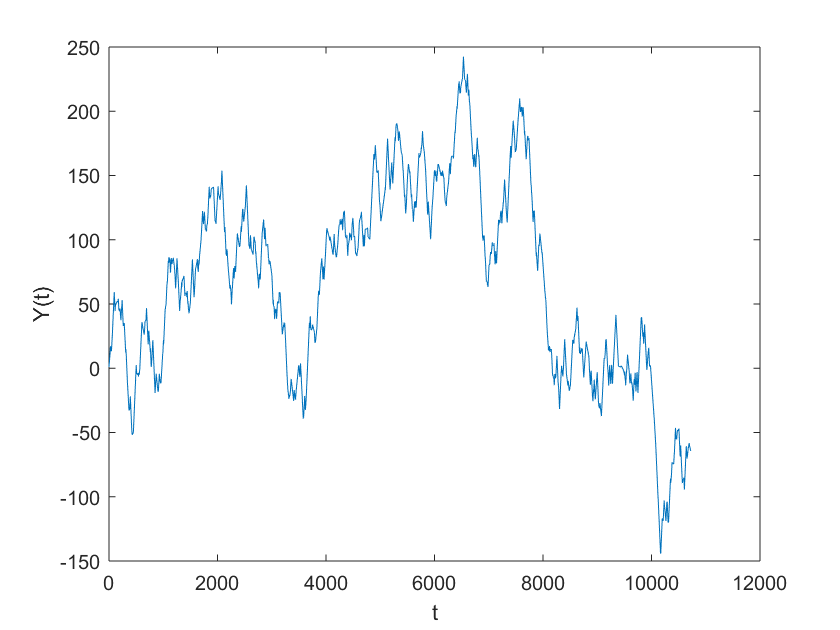
\includegraphics[scale=0.4]{images/N1000T1n10.png}
     \caption{Figure 1}\label{fig:figA}
   \end{subfigure}
   \begin{subfigure}{0.6\linewidth} \centering
     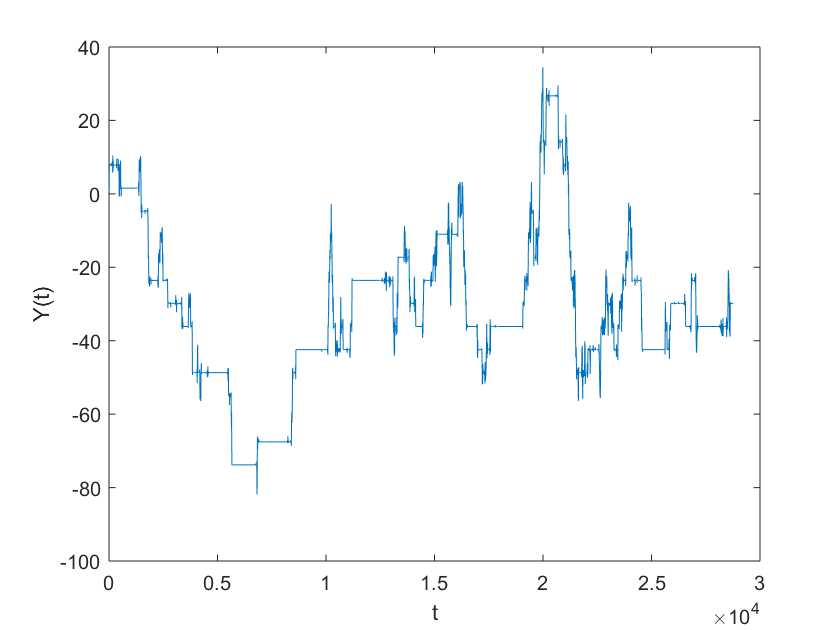
\includegraphics[scale=0.4]{images/N10000T70n20.png}
     \caption{Figure 2}\label{fig:figB}
   \end{subfigure}
\caption{Trajectories of the numerical solution obtained by the Euler-Poisson Scheme} \label{fig:twofigs}
\end{figure}

%We simulated the Euler-Poisson scheme \eqref{eq5} 1000 times sampling from the distribution of $\Delta X_{\xi_{i}(n/T)}$ and chose $a(x)= \sin{(x)}$ arbitrarily with $T=1$, $n=10$.

% \noindent
% Some cross-references: First, we refer to Figure~\ref{fig:twofigs}. 
% Second, we can also refer to the component figures individually, 
% viz., to Figures~\ref{fig:figA} and \ref{fig:figB}.
% \begin{figure}[h]
% \caption{Trajectories of the Euler-Poisson Scheme}
% \centering
% 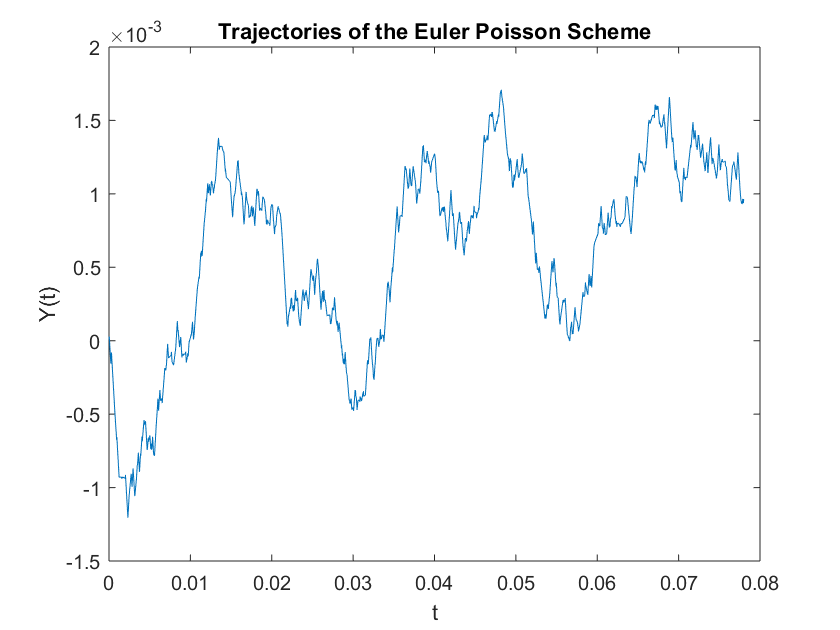
\includegraphics[width=1\textwidth]{images/1000.png}
% \end{figure}

% \begin{figure}[h]
% \caption{Trajectories of the Euler-Poisson Scheme}
% \centering
% 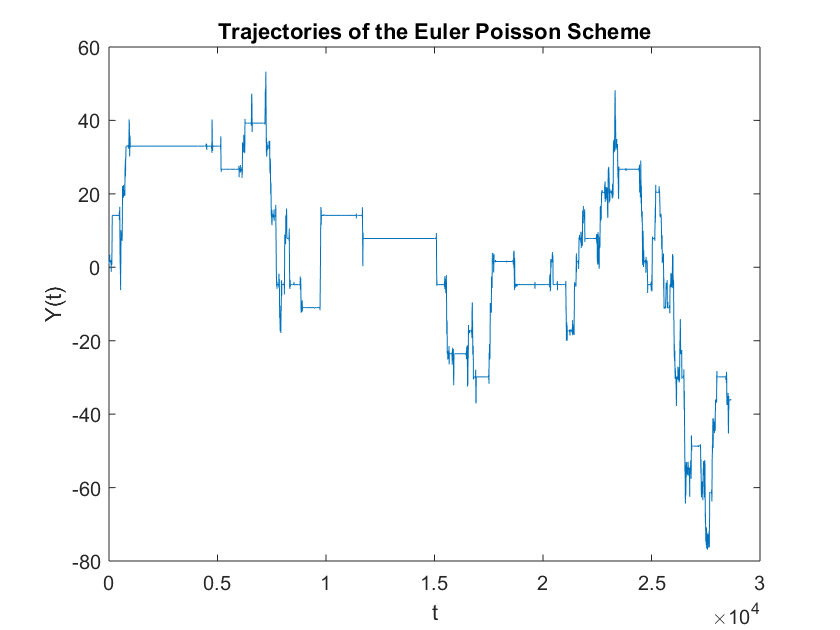
\includegraphics[width=1\textwidth]{images/unscaledN10000T70n20.png}
% \end{figure}



%\appendix
\begin{appendices}
\chapter*{Appendix}
\section{Standard Inequalities}
\subsection{Gronwall's Inequality}
\begin{theorem}\label{Append_Gron_ineq}
Let $\alpha$ and $f$ be nonnegative, continuous functions defined for $t \in [0, \, T]$, and let $\mathbf{C}_0 \geq 0$ denote a constant. If
\begin{equation}
    \alpha(t) \leq \mathbf{C}_0 + \int^t_0 f \alpha ds, \qquad\qquad for \, all \quad t \in [0, \, T],
\end{equation}
then
\begin{equation}
    \alpha(t) \leq \mathbf{C}_0 e^{\int^t_0 f ds}, \qquad\qquad for \, all \quad t \in [0, \, T].
\end{equation}
\end{theorem}
\begin{proof}
Set 
\begin{equation*}
    \beta(t) :=  \mathbf{C}_0 + \int^t_0 f \alpha ds.
\end{equation*}
Then $\beta^\prime = f \alpha \leq f \beta$, and so
\begin{equation*}
    \bigg(\beta \, e^{-\int^t_0 f ds}\bigg)^\prime = (\beta^\prime - f \beta)e^{-\int^t_0 f ds} \leq (f \alpha - f \alpha)e^{-\int^t_0 f ds} = 0.
\end{equation*}
Therefore 
\begin{equation*}
    \beta (t) e^{-\int^t_0 f ds} \leq \beta (0) e^{-\int^t_0 f ds} = \mathbf{C}_0,
\end{equation*}
and thus 
\begin{equation*}
    \alpha(t) \leq \beta(t) \leq \mathbf{C}_0 e^{-\int^t_0 f ds}.
\end{equation*}
\end{proof}


\subsection{Doob's Inequality}
\begin{theorem}
Let $(M_t)_{t \geq 0}$ be a continuous martingale with respect to the filtration $(\mathcal{F}_t)_{t \geq 0}$ defined on $(\Omega , \mathcal{F}, \mathcal{P})$. If $p > 1$, $T > 0$ and  $\mathbb{E}[|M_T|^p] \leq +\infty$, then we have that
\begin{equation}\label{Append_Doob_ineq}
    \mathbb{E}\big[\sup_{t \in [0, \, T]}|M_t|^p\big]  \leq \bigg( \dfrac{p}{p-1}\bigg)\mathbb{E}[|M_T|^p].
\end{equation}
\end{theorem}
\begin{proof}
See \morecite{protter2005stochastic}, Theorem 74, p. 226.
\end{proof}
%https://fabricebaudoin.wordpress.com/2012/04/10/lecture-11-doobs-martingale-maximal-inequalities/
\subsection{Cauchy-Schwartz Inequality}
The following which is an implication of the Cauchy-Schwartz Inequality taken from \morecite{choe2016stochastic}.
\begin{theorem}
Let $g : [0, t] \to \mathbb{R}^n$. For any $t > 0 $ we have that 
\begin{equation}\label{Appendix_CS}
    \bigg| \int^t_0 g \, ds  \bigg|^2 \leq t \int^t_0 |g|^2 ds.
\end{equation}
\end{theorem}


\section{Simulation Code}
\lstinputlisting{images/EP.m}
\end{appendices}
%\addcontentsline{toc}{section}{Appendices}

%\addcontentsline{toc}{chapter}{Appendix}
%\input{erklaer}
%\input{chapter_5}
%\input{chapter_4}





${ } $



%\pagenumbering{arabic}
%\setcounter{page}{1} \normalsize

%%%%%%%%%%%%%%%%%%%%%%%%%%%%%%%%%%%%%%
%%%%%%%%%%%%%%%%%%%%%%%%%%%%%%%%%%%%%%
%%%%%%%%%%%%%%%%%%%%%%%%%%%%%%%%%%%%%%
%\input{chapter_1}
%\input{kapitel7}
%\input{kapitel8}
%\input{kapitel9}
%\setcounter{chapter}{9}
%\nocite{*}
\addcontentsline{toc}{chapter}{Bibliography}
\printbibliography
\chapter*{Declaration}
I declare that I have authored this thesis independently, that I have not used other than the declared sources, and that I have explicitly marked all material which has been quoted either literally or by content from the used sources. I furthermore declare that this thesis has not been submitted to any other board of examiners yet.

\end{document}
